%%%%%%%%%%%%%%%%%%%%%%%%%%%%%%%%%%%%%%%%%%%%%%%%%%%%%%%%%%%%%%%%%%%%%%
% Overleaf (WriteLaTeX) Example: Molecular Chemistry Presentation
%
% Source: http://www.overleaf.com
%
% In these slides we show how Overleaf can be used with standard
% chemistry packages to easily create professional presentations.
%
% Feel free to distribute this example, but please keep the referral
% to overleaf.com
%
%%%%%%%%%%%%%%%%%%%%%%%%%%%%%%%%%%%%%%%%%%%%%%%%%%%%%%%%%%%%%%%%%%%%%%

\documentclass[xcolor={dvipsnames}]{beamer}

\mode<presentation>
{
  \usetheme{Madrid}       % or try default, Darmstadt, Warsaw, ...
  \usecolortheme{default} % or try albatross, beaver, crane, ...
  \usefonttheme{default}    % or try default, structurebold, ...
  \setbeamertemplate{navigation symbols}{}
  \setbeamertemplate{caption}[numbered]
}

\usepackage[english]{babel}
\usepackage[utf8x]{inputenc}
\usepackage{graphicx}
\usepackage{hyperref}
  \hypersetup{colorlinks=true}
  \hypersetup{urlcolor=blue}
  \hypersetup{linkcolor = .}
\usepackage{xcolor}
\usepackage{siunitx}
  \sisetup{separate-uncertainty = true}
\DeclareSIUnit\barn{b}
\usepackage{physics}
\usepackage[font=small,labelfont=bf]{caption}
\usepackage{subcaption}
\usepackage[en-GB]{datetime2}
\usepackage{overpic}
\usepackage{feynmp}
\DeclareGraphicsRule{*}{mps}{*}{}
\usepackage{scalerel}
\newcommand{\mylbrace}[2]{\vspace{#2pt}\hspace{6pt}\scaleleftright[\dimexpr5pt+#1\dimexpr0.06pt]{\lbrace}{\rule[\dimexpr2pt-#1\dimexpr0.5pt]{-4pt}{#1pt}}{.}}
\newcommand{\myrbrace}[2]{\vspace{#2pt}\scaleleftright[\dimexpr5pt+#1\dimexpr0.06pt]{.}{\rule[\dimexpr2pt-#1\dimexpr0.5pt]{-4pt}{#1pt}}{\rbrace}\hspace{6pt}}

% Trim in percent
\usepackage{adjustbox}

% No "Figure" prefix
\setbeamertemplate{caption}{\raggedright\insertcaption\par}

% Nice decay amplitude diagrams
\usepackage{amsmath,amssymb,tikz-cd}

% Strike out text
\usepackage[normalem]{ulem}

% For figures with text overlay
\usepackage{overpic}

% Arrows
\usepackage{tikz}
\newcommand{\tikzmark}[1]{\tikz[remember picture] \node[coordinate] (#1) {#1};}

% Colourbox with line breaks
\newcommand{\cbox}[2][lime!20]{%
  \colorbox{#1}{\parbox{\dimexpr\linewidth-2\fboxsep}{\strut #2\strut}}%
}

% Vector arrows
\usepackage[pdftex]{pict2e}

% Checkmark symbol
\def\checkmark{\tikz\fill[scale=0.4](0,.35) -- (.25,0) -- (1,.7) -- (.25,.15) -- cycle;}

% Here's where the presentation starts, with the info for the title slide
\title[Heidelberg tracking meeting]{Understanding discrepancies in tracking efficiencies}

\author[Martin Tat]{Martin Tat}
\institute[Heidelberg]{Heidelberg University}
\date{16th July 2025}

\titlegraphic{
\includegraphics[height = 2.3cm]{lhcb.jpg}\hspace{1.0cm}~%
              
\includegraphics[height = 2.3cm]{HeidelbergLogo.pdf}}

\begin{document}

\begin{frame}
  \titlepage
\end{frame}

% These three lines create an automatically generated table of contents.
%\begin{frame}{Outline}
%  \tableofcontents
%\end{frame}

\begin{frame}{Introduction}
  \vspace{0.0cm}
  {\Large I have had a look at the work on tracking efficiencies by Rowina and Maurice}
  \vspace{0.2cm}
  \begin{itemize}
    \setlength\itemsep{0.8em}
    \item{Some discrepancy between different tag-and-probe methods:}
    \begin{enumerate}
      \item{Combined: VeloMuon $\times$ Downstream}
      \begin{itemize}
        \item{VeloMuon: Determine SciFi efficiency}
        \item{Downstream: Determine Velo efficiency}
      \end{itemize}
      \item{MuonUT: Determine long track efficiency}
    \end{enumerate}
    \item{Presentation today:}
    \begin{enumerate}
      \item{I have looked at this with fresh eyes, and I have some ideas about what to study in more detail}
      \begin{itemize}
        \item{Thanks to Rowina for a well written thesis, which simplifies this detective work}
      \end{itemize}
      \item{Today I will show work produced by TrackCalib2}
      \begin{itemize}
        \item{Thanks for Maurice for all the assistance}
      \end{itemize}
      \item{Specifically, today I will show some studies on fit biases}
    \end{enumerate}
  \end{itemize}
\end{frame}

\begin{frame}{Tag-and-probe method}
  \vspace{0.0cm}
  \begin{figure}[htb]
    \centering
    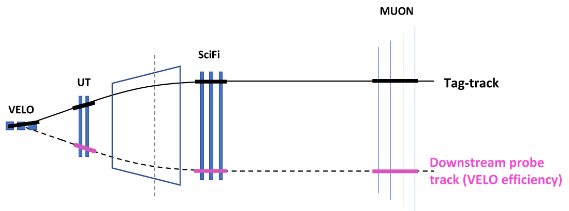
\includegraphics[width=0.75\textwidth]{Plots/Tag_and_probe_method.png}
    \caption*{\small Figure from \href{https://www.physi.uni-heidelberg.de/Publications/PhD_thesis.pdf}{Rowina's thesis}}
  \end{figure}
  \begin{itemize}
    \item{Fully reconstruct one muon from $J/\psi\to\mu^+\mu^-$}
    \item{Partially reconstruct the other muon}
    \item{Match hits in specific sub-detector with partially reconstructed track}
  \end{itemize}
  \begin{equation*}
    \epsilon_{\rm track} = \frac{N_{\rm matched}}{N_{\rm matched} + N_{\rm failed}}
  \end{equation*}
\end{frame}

\begin{frame}{TrackCalib2}
  \vspace{0.0cm}
  \begin{figure}[htb]
    \centering
    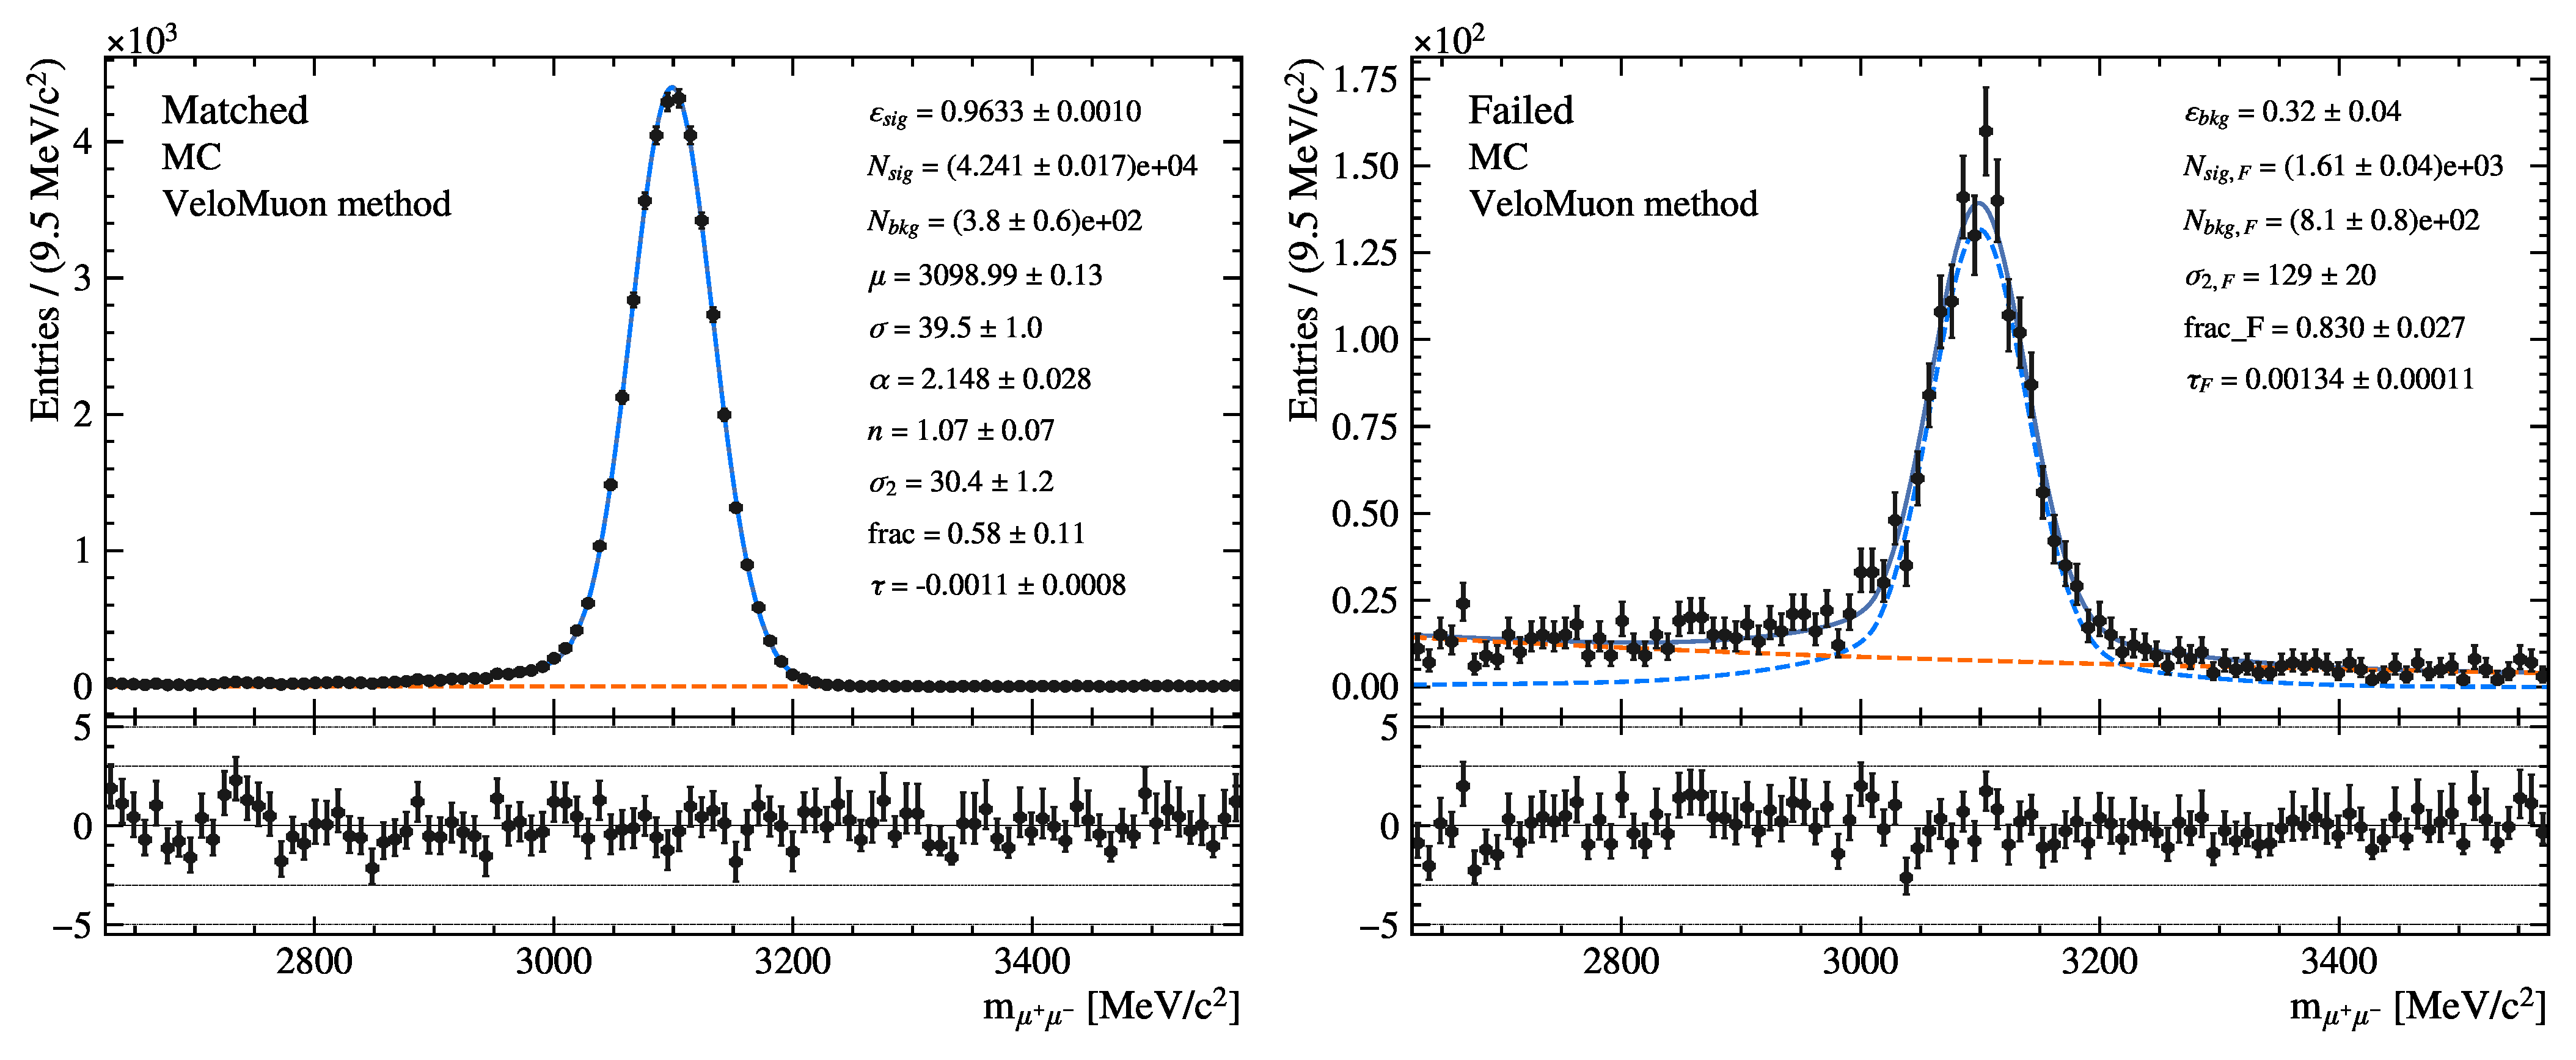
\includegraphics[width=1.0\textwidth]{Plots/MC_VeloMuon_P_bin_0_ETA_bin_0_sim.pdf}
    \caption*{\small VeloMuon $(p, \eta)$ bin $(0, 0)$}
  \end{figure}
  \vspace{-0.5cm}
  \begin{itemize}
    \item{I tried running the default fits with TrackCalib2 on MC...}
    \item{... and things are working more or less out-of-the-box!}
    \item{The fit outputs $\epsilon_{\rm track}$ directly as a fit parameter}
  \end{itemize}
\end{frame}

\begin{frame}{TrackCalib2}
  \vspace{0.0cm}
  \begin{figure}[htb]
    \centering
    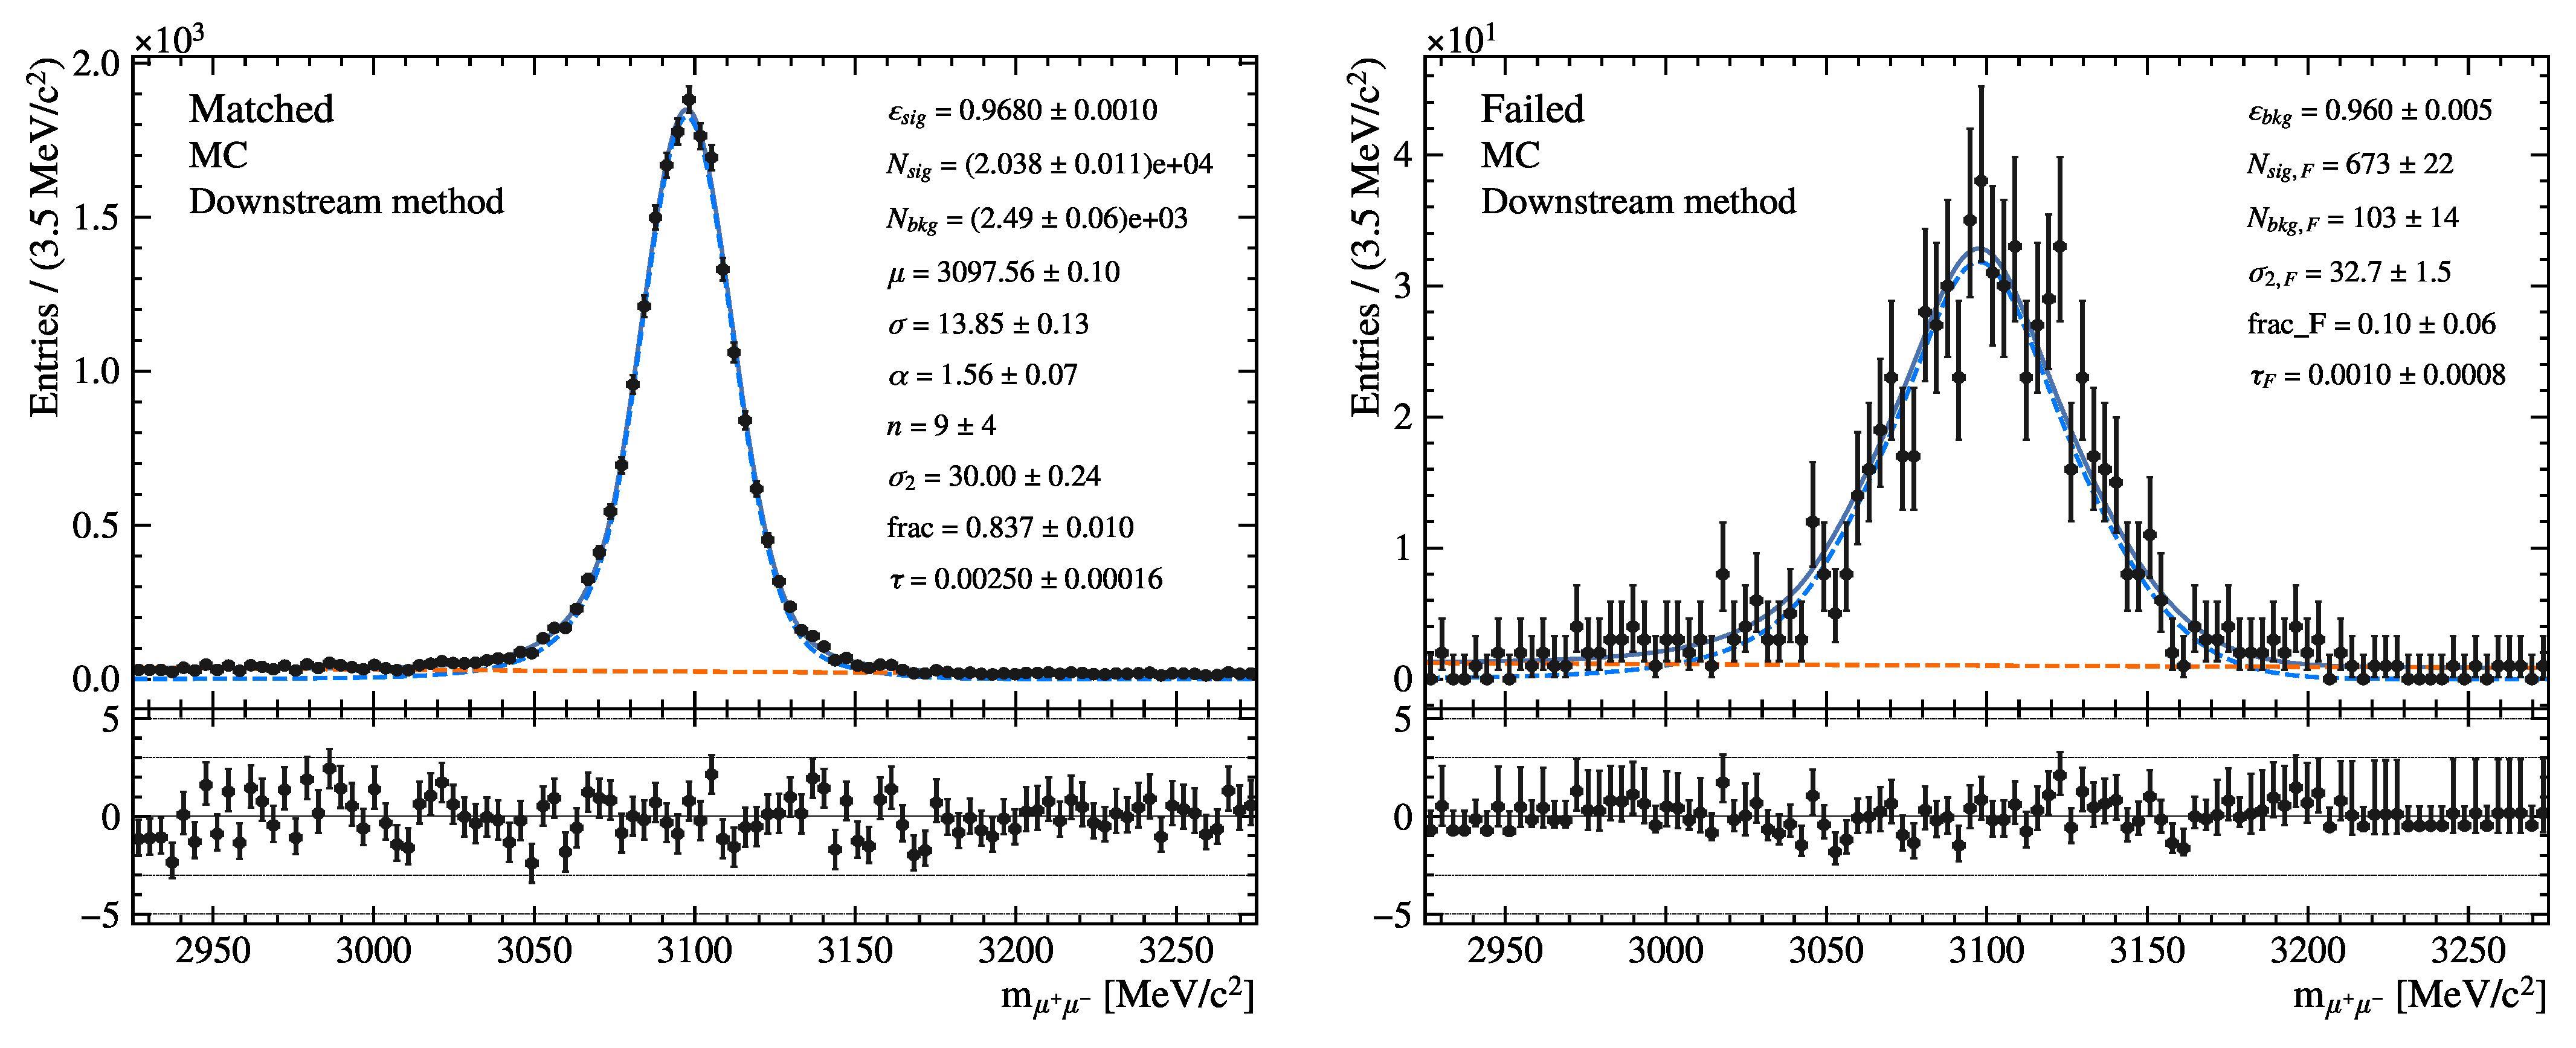
\includegraphics[width=1.0\textwidth]{Plots/MC_Downstream_P_bin_0_ETA_bin_0_sim.pdf}
    \caption*{\small Downstream $(p, \eta)$ bin $(0, 0)$}
  \end{figure}
  \vspace{-0.5cm}
  \begin{itemize}
    \item{I tried running the default fits with TrackCalib2 on MC...}
    \item{... and things are working more or less out-of-the-box!}
    \item{The fit outputs $\epsilon_{\rm track}$ directly as a fit parameter}
  \end{itemize}
\end{frame}

\begin{frame}{TrackCalib2}
  \vspace{0.0cm}
  \begin{figure}[htb]
    \centering
    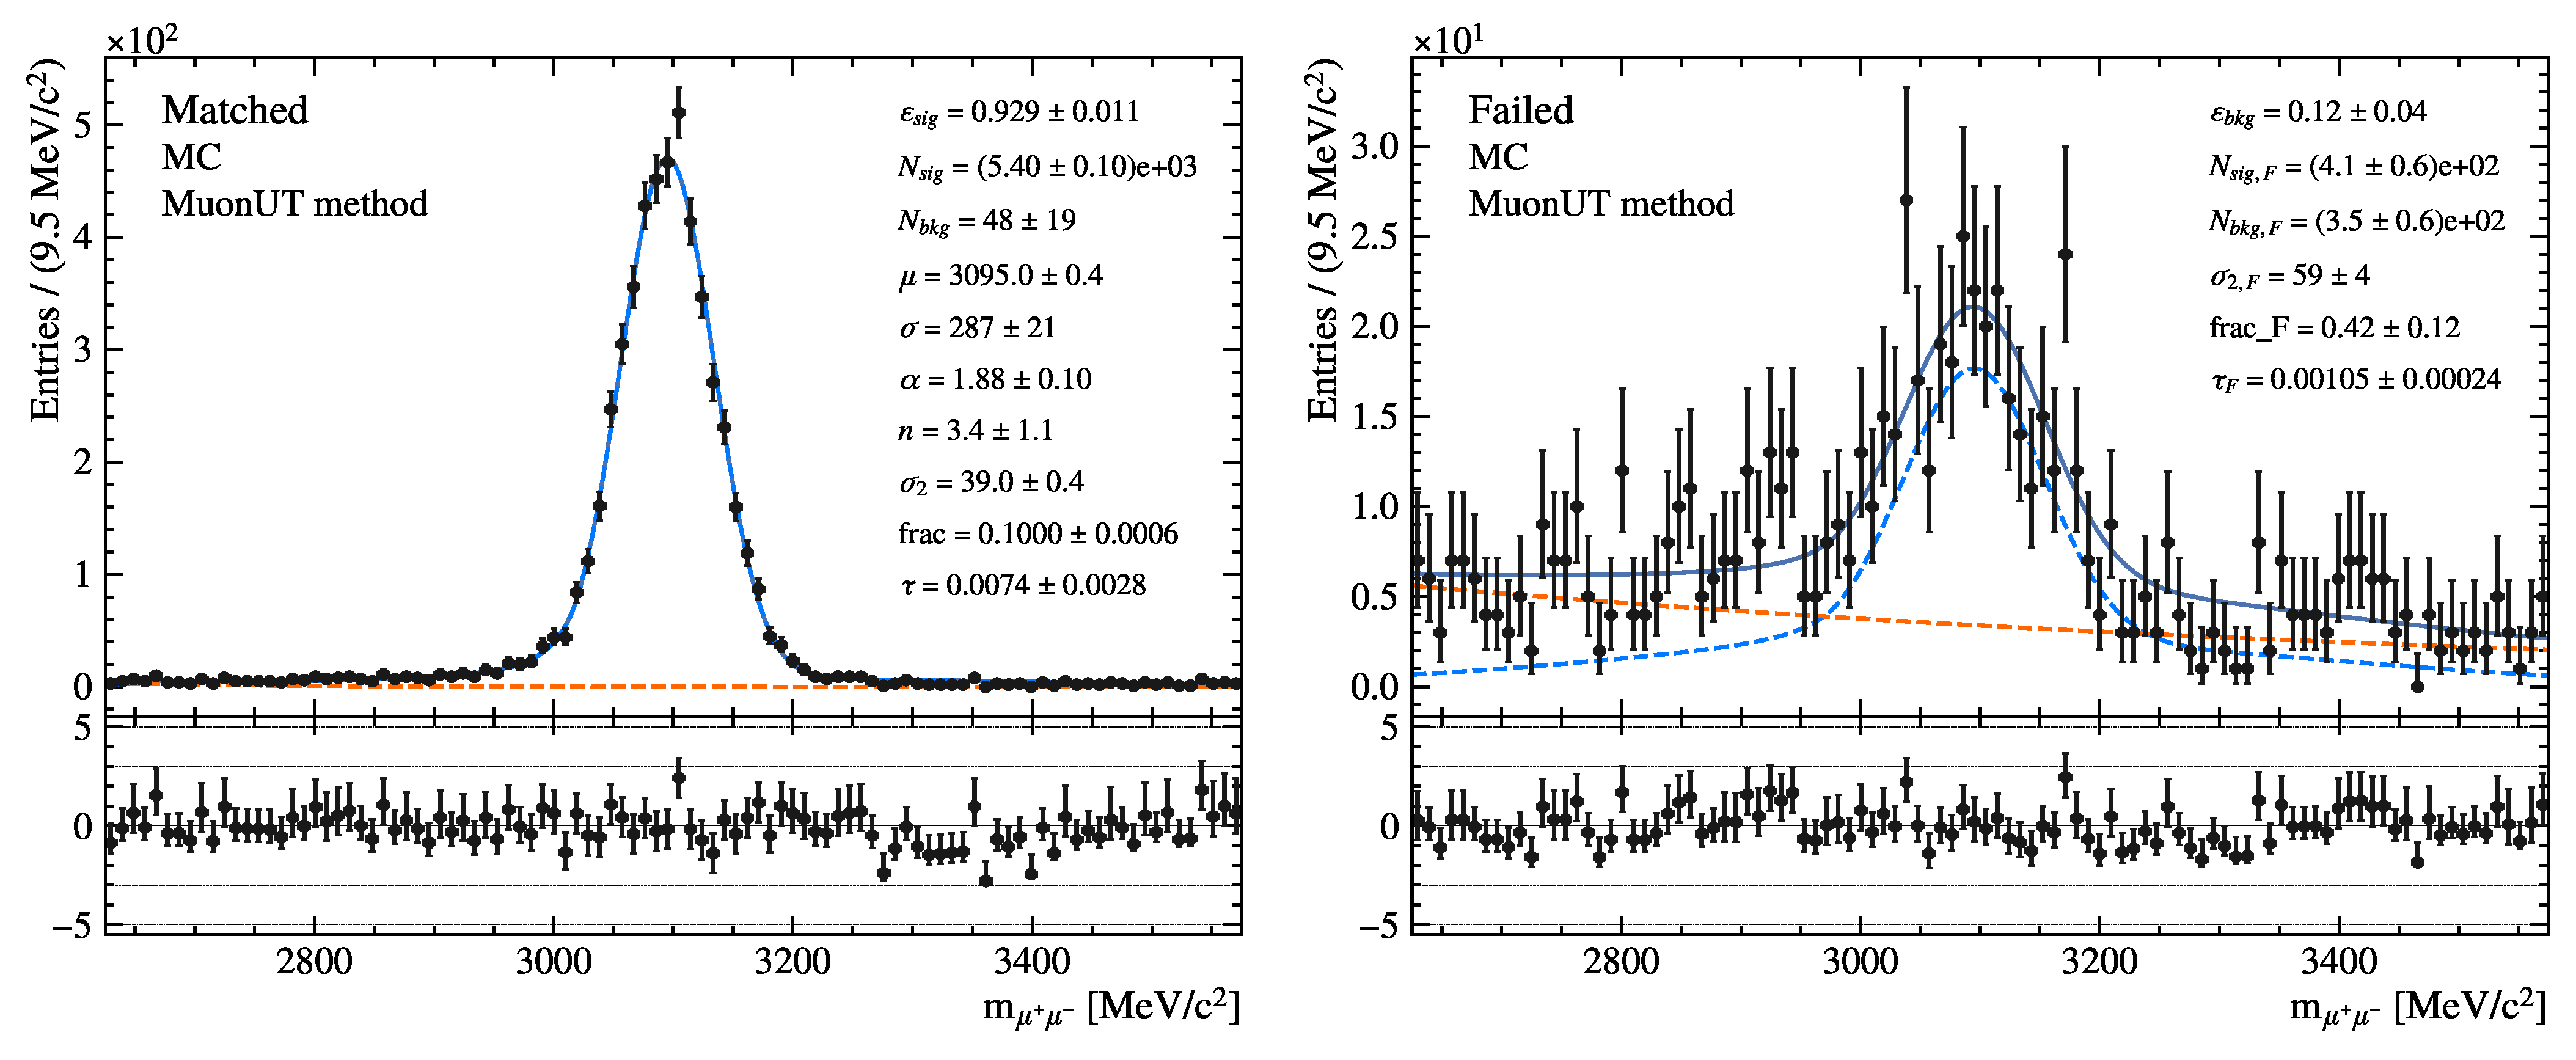
\includegraphics[width=1.0\textwidth]{Plots/MC_MuonUT_P_bin_0_ETA_bin_0_sim.pdf}
    \caption*{\small MuonUT $(p, \eta)$ bin $(0, 0)$}
  \end{figure}
  \vspace{-0.5cm}
  \begin{itemize}
    \item{I tried running the default fits with TrackCalib2 on MC...}
    \item{... and things are working more or less out-of-the-box!}
    \item{The fit outputs $\epsilon_{\rm track}$ directly as a fit parameter}
  \end{itemize}
\end{frame}

\begin{frame}{TrackCalib2}
  \vspace{0.0cm}
  \begin{figure}[htb]
    \centering
    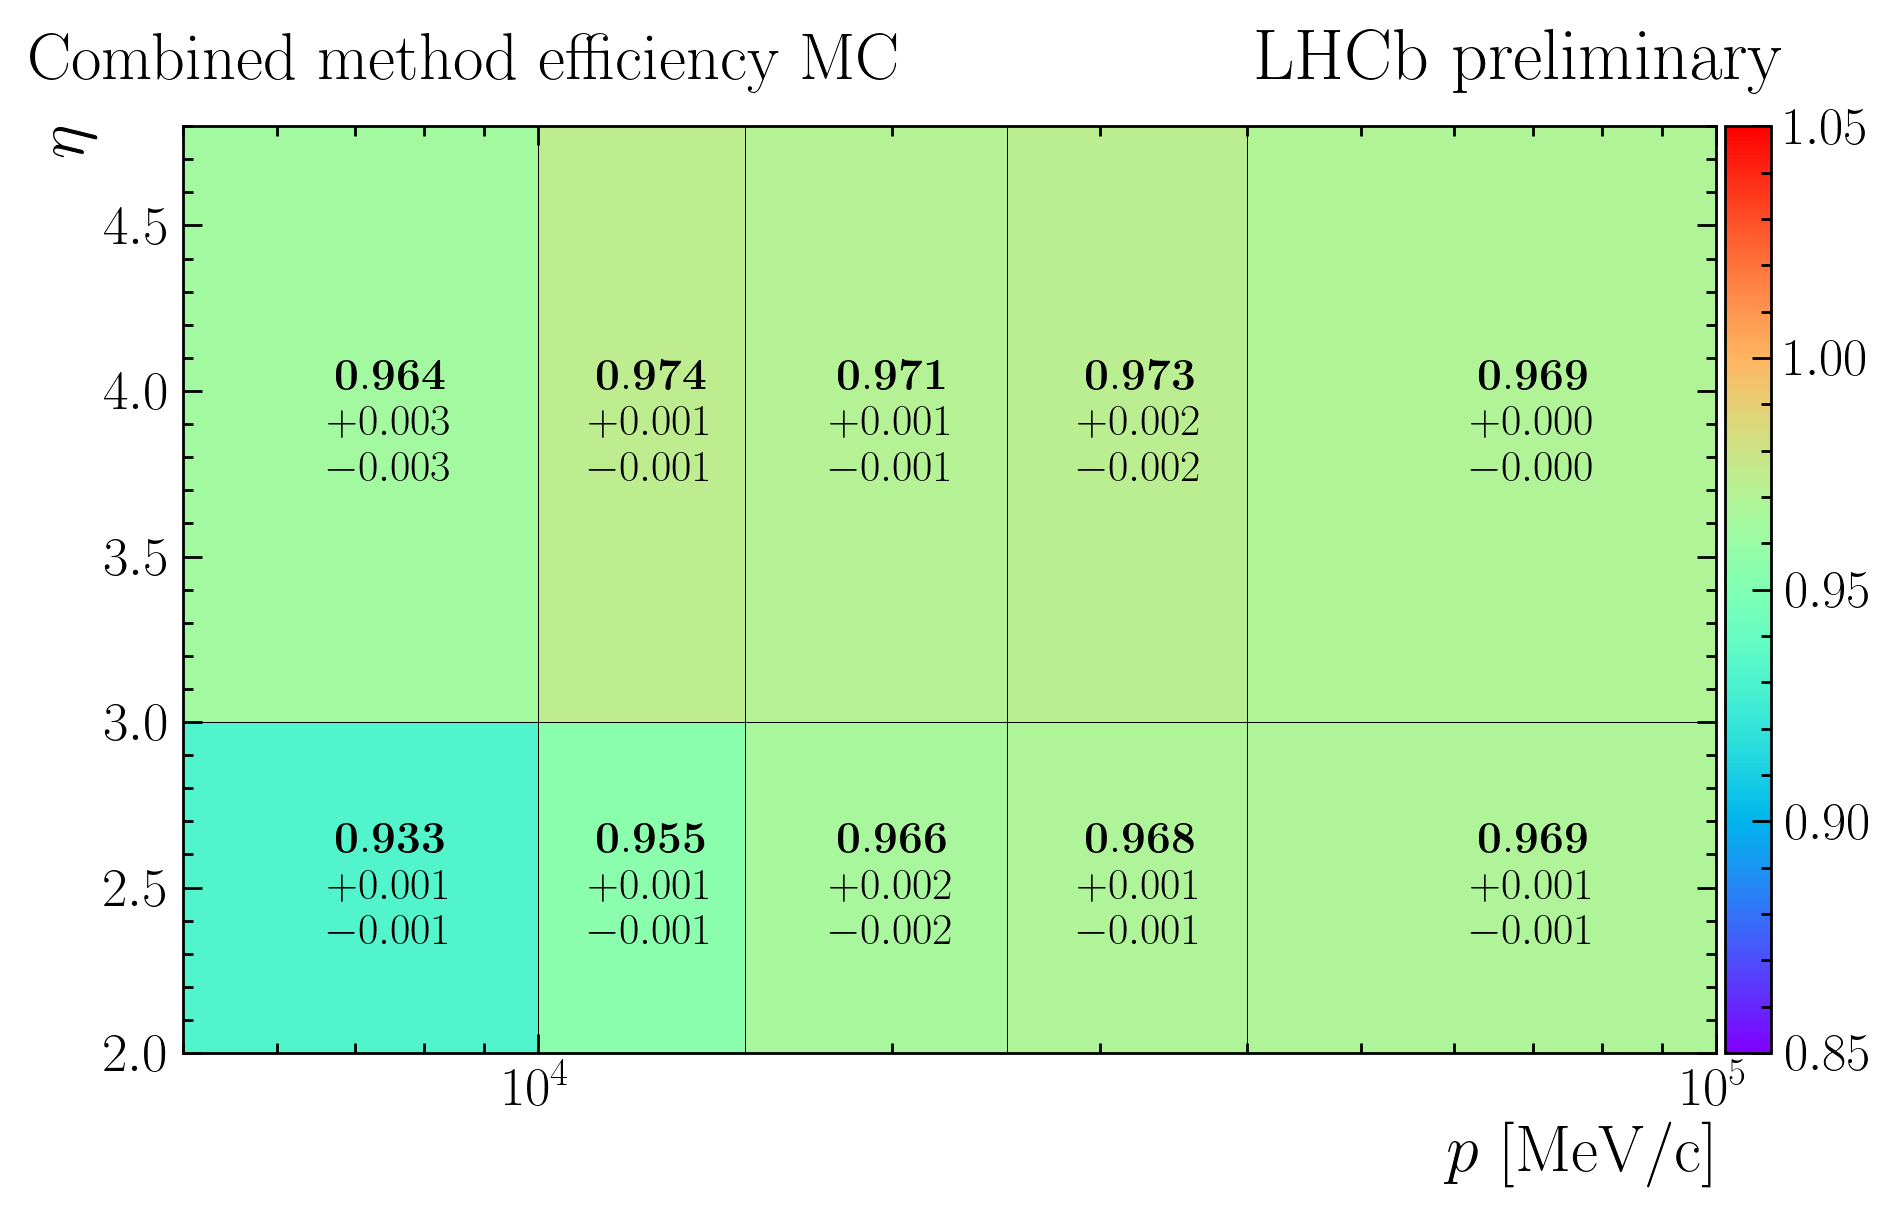
\includegraphics[width=0.9\textwidth]{Plots/trackEff_MC_Sim10d_2024_Block1_Combined_P-ETA.png}
    \caption*{\small Track efficiencies with Combined method produced by TrackCalib2}
  \end{figure}
\end{frame}

\begin{frame}{TrackCalib2}
  \vspace{0.0cm}
  \begin{figure}[htb]
    \centering
    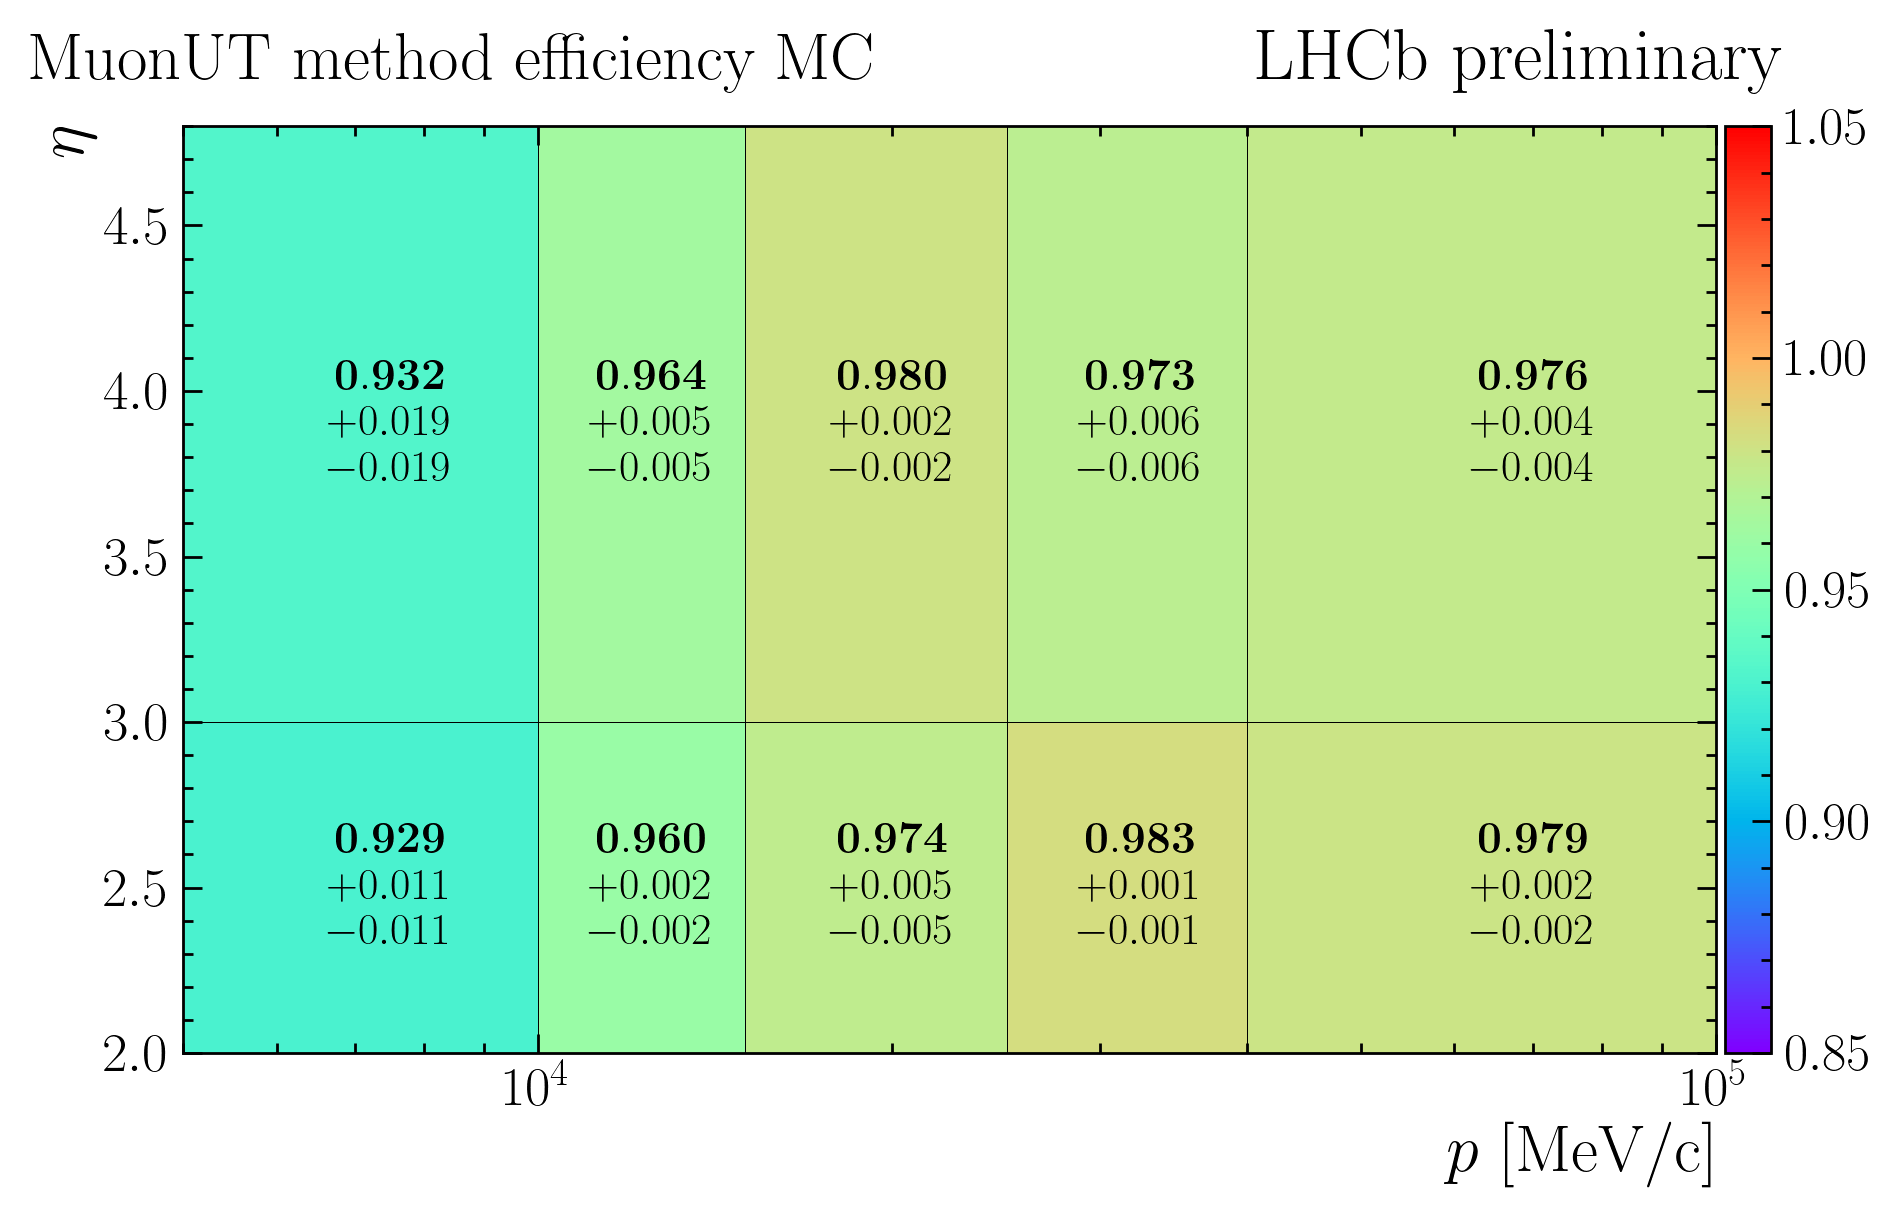
\includegraphics[width=0.9\textwidth]{Plots/trackEff_MC_Sim10d_2024_Block1_MuonUT_P-ETA.png}
    \caption*{\small Track efficiencies with MuonUT method produced by TrackCalib2}
  \end{figure}
\end{frame}

\begin{frame}{Track efficiencies}
  \vspace{0.0cm}
  \begin{center}
    Some discrepancies found...:
  \end{center}
  \begin{center}
    \begin{tabular}{ccc}
      \hline
      $p$ bin & $\eta$ bin & Difference ($10^{-2}$) \\
      \hline
      $0$     & $0$        & $\phantom{-}0.4 \pm 1.1$ \\
      $1$     & $0$        & $-0.5 \pm 0.2$ \\
      $2$     & $0$        & $-0.8 \pm 0.5$ \\
      $3$     & $0$        & $-1.5 \pm 0.1$ \\
      $4$     & $0$        & $-1.0 \pm 0.2$ \\
      $0$     & $1$        & $\phantom{-}3.2 \pm 1.9$ \\
      $1$     & $1$        & $\phantom{-}1.0 \pm 0.5$ \\
      $2$     & $1$        & $-0.9 \pm 0.2$ \\
      $3$     & $1$        & $\phantom{-}0.0 \pm 0.6$ \\
      $4$     & $1$        & $-0.7 \pm 0.4$ \\
      \hline
    \end{tabular}
  \end{center}
\end{frame}

\begin{frame}{Discrepancies in track efficiencies}
  \vspace{0.0cm}
  \begin{center}
    Do we care about these discrepancies?
  \end{center}
  \begin{itemize}
    \setlength\itemsep{1.0em}
    \item{Yes: Some are statistically significantly different from zero}
    \item{No: Method is not perfect, expect $\mathcal{O}(1\%)$ differences}
    \item{Yes: We want to keep systematics under control (roughly $2\%$)}
    \item{No: Most of the differences are around $1\%$, except for one bin with a large uncertainty}
  \end{itemize}
\end{frame}

\begin{frame}{Fitting the track efficiency}
  \vspace{0.0cm}
  \begin{equation*}
    \epsilon_{\rm track} = \frac{N_{\rm matched}}{N_{\rm matched} + N_{\rm failed}}
  \end{equation*}
  \begin{itemize}
    \setlength\itemsep{1.0em}
    \item{Fit total yield $N_{\rm tot} = N_{\rm matched} + N_{\rm failed}$ and $\epsilon_{\rm track}$ directly}
    \item{$N_{\rm tot}$ and $\epsilon_{\rm track}$ can be related to the yields:}
  \end{itemize}
  \vspace{-0.2cm}
  \begin{align*}
    N_{\rm matched} =& N_{\rm tot}\times\epsilon_{\rm track} \\
    N_{\rm failed} =& N_{\rm tot}\times(1 - \epsilon_{\rm track})
  \end{align*}
  \vspace{-0.5cm}
  \begin{itemize}
    \item{An analogous set of parameters exist for the background yields}
    \item{My suspicion: $\epsilon_{\rm track}\in[0, 1]$, but $\epsilon_{\rm track}$ is close to $1$}
    \begin{itemize}
      \item[-]{Maximum-likelihood fit might be biased}
      \item[-]{Particularly important then $N_{\rm failed}\approx 0$}
    \end{itemize}
    \item{Generate toys to assess this effect}
    \item{For now, only check MuonUT method as the yields are lower}
  \end{itemize}
\end{frame}

\begin{frame}{Fit biases}
  \vspace{0.0cm}
  \begin{figure}[htb]
    \centering
    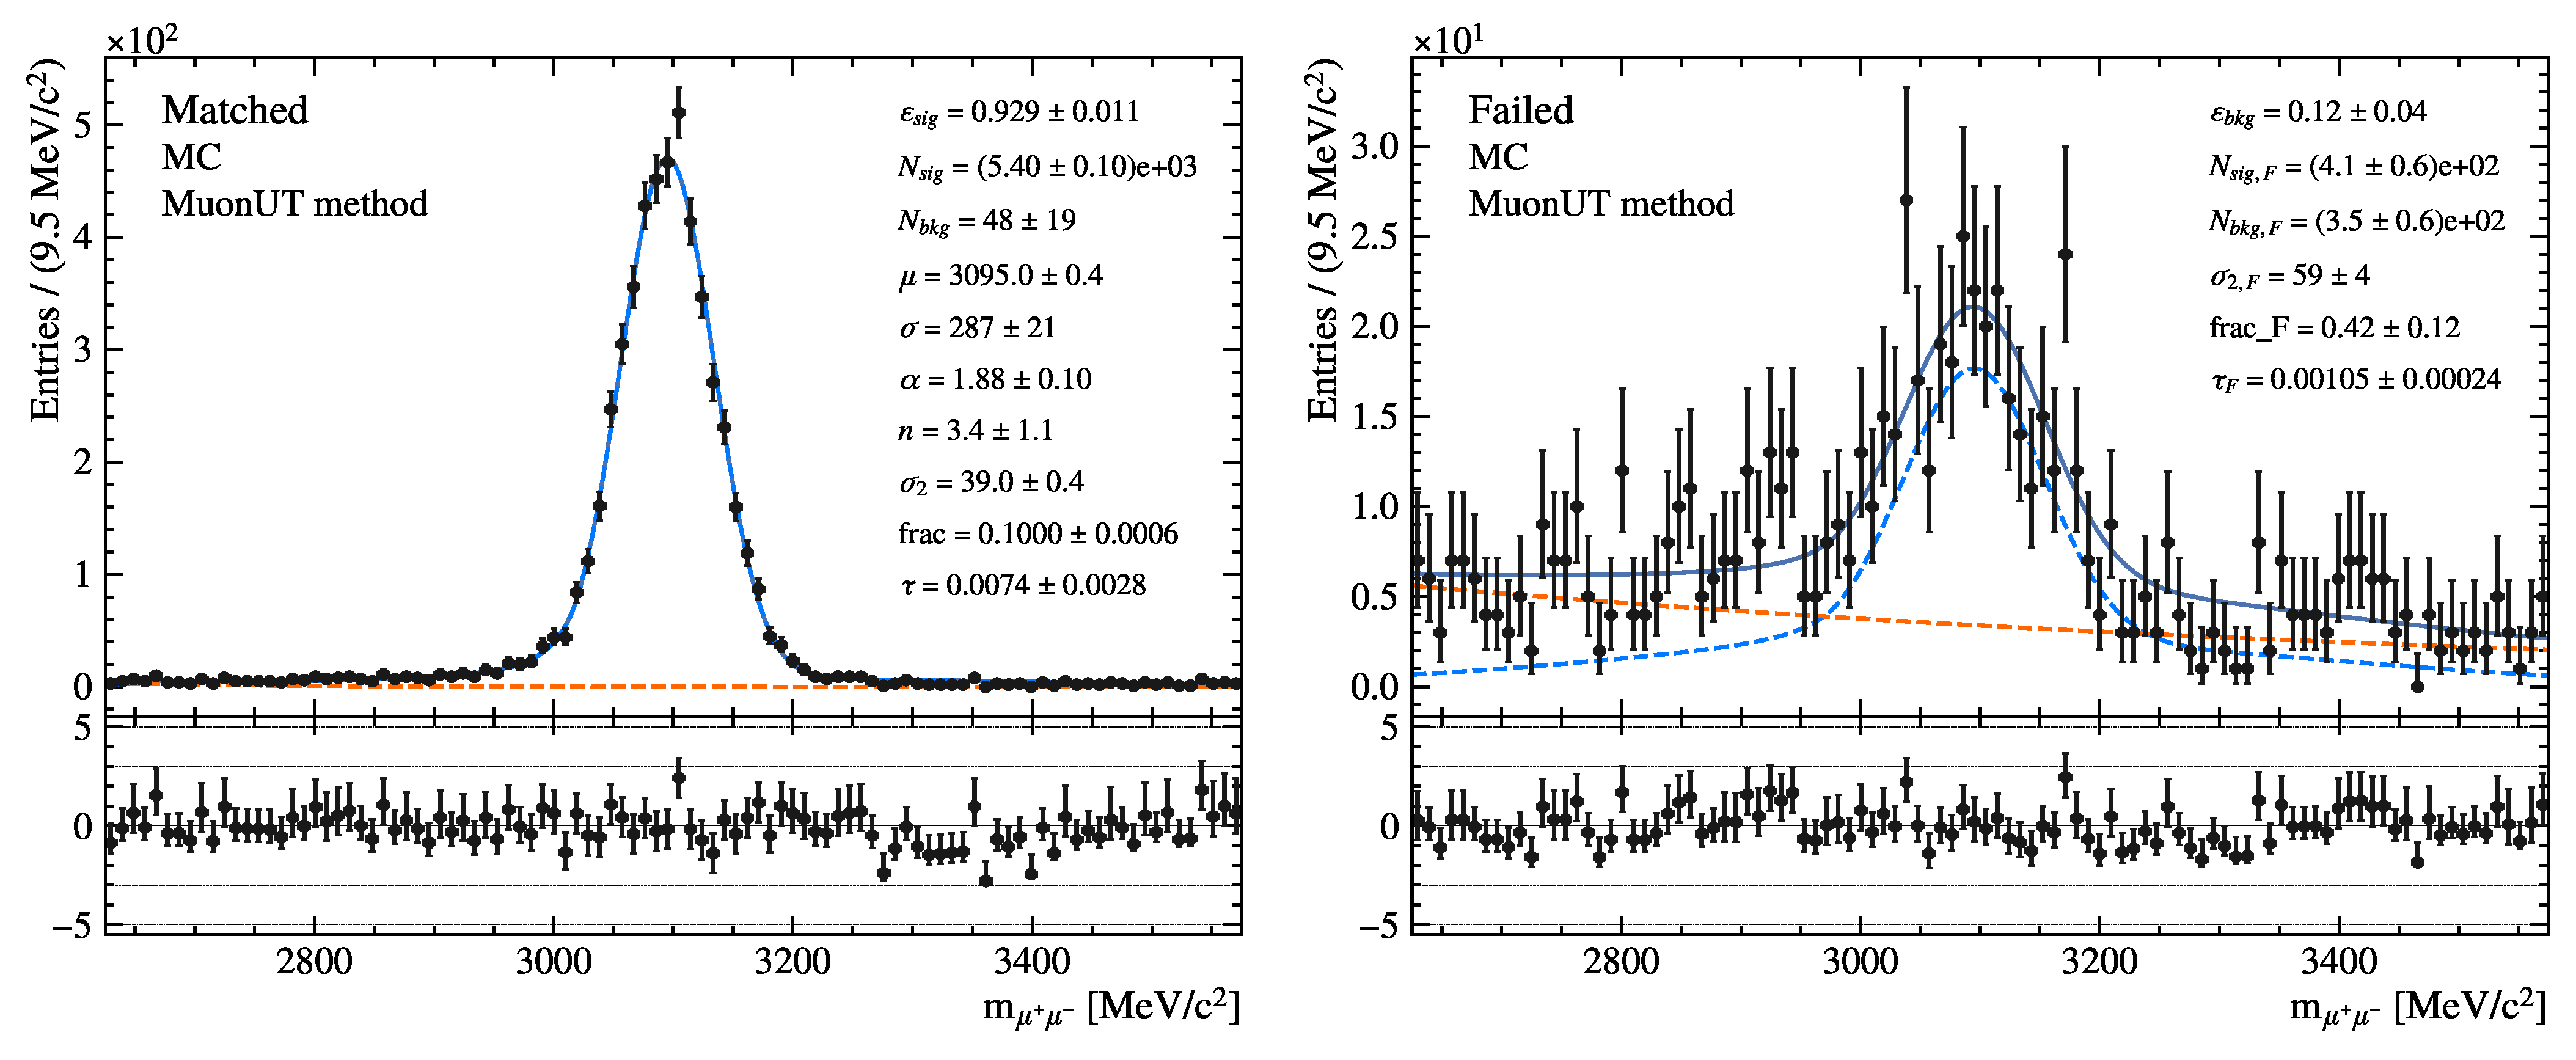
\includegraphics[width=0.7\textwidth]{Plots/MC_MuonUT_P_bin_0_ETA_bin_0_sim.pdf}
    \caption*{\small MuonUT $(p, \eta)$ bin $(0, 0)$ MC fit}
  \end{figure}
  \vspace{-0.5cm}
  \begin{figure}[htb]
    \centering
    \begin{subfigure}{0.45\textwidth}
      \centering
      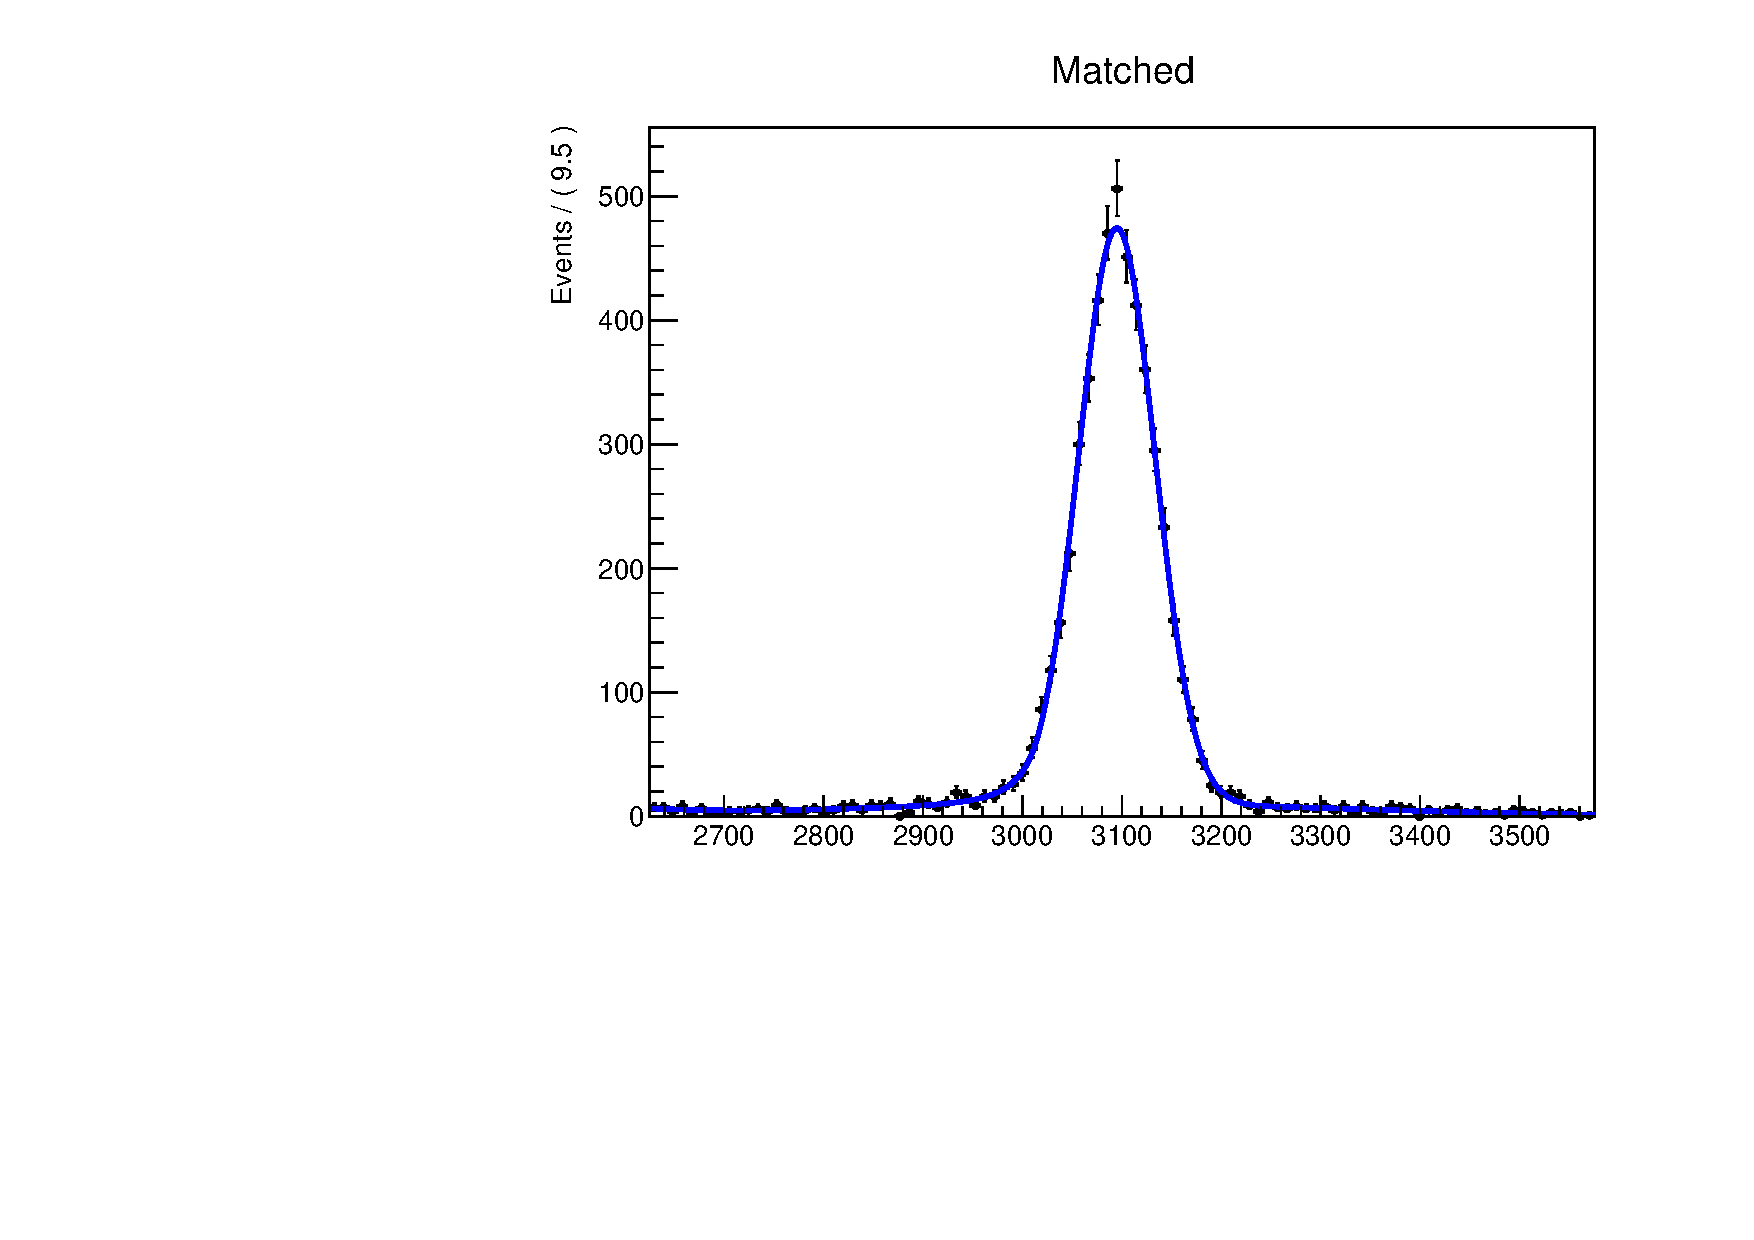
\includegraphics[width=0.8\textwidth]{Plots/matched_projection_MuonUT_P0_ETA0.pdf}
    \end{subfigure}%
    \begin{subfigure}{0.45\textwidth}
      \centering
      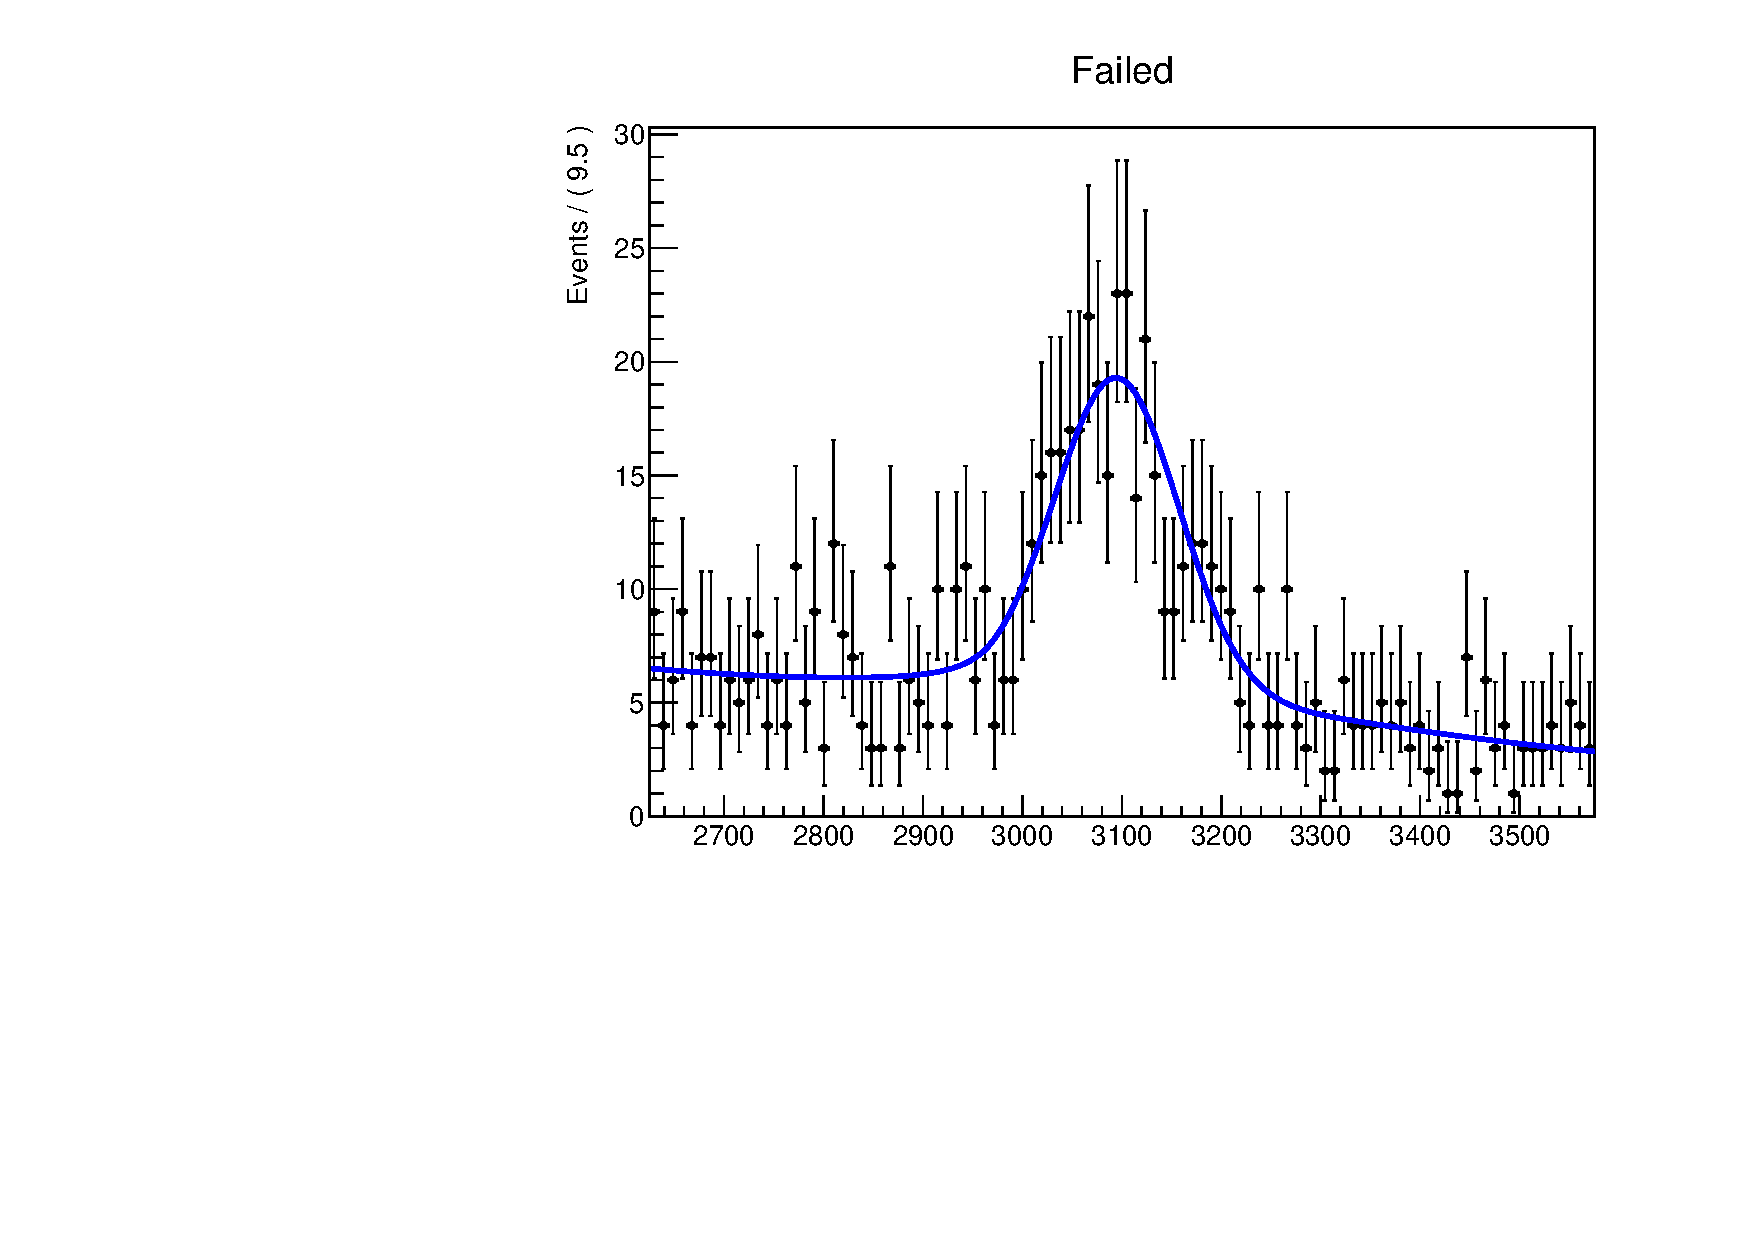
\includegraphics[width=0.8\textwidth]{Plots/failed_projection_MuonUT_P0_ETA0.pdf}
    \end{subfigure}
    \vspace{-0.2cm}
    \caption*{\small MuonUT $(p, \eta)$ bin $(0, 0)$ toy fit}
  \end{figure}
\end{frame}

\begin{frame}{Well-behaved fits}
  \vspace{0.0cm}
  \begin{figure}[htb]
    \centering
    \begin{subfigure}{0.45\textwidth}
      \centering
      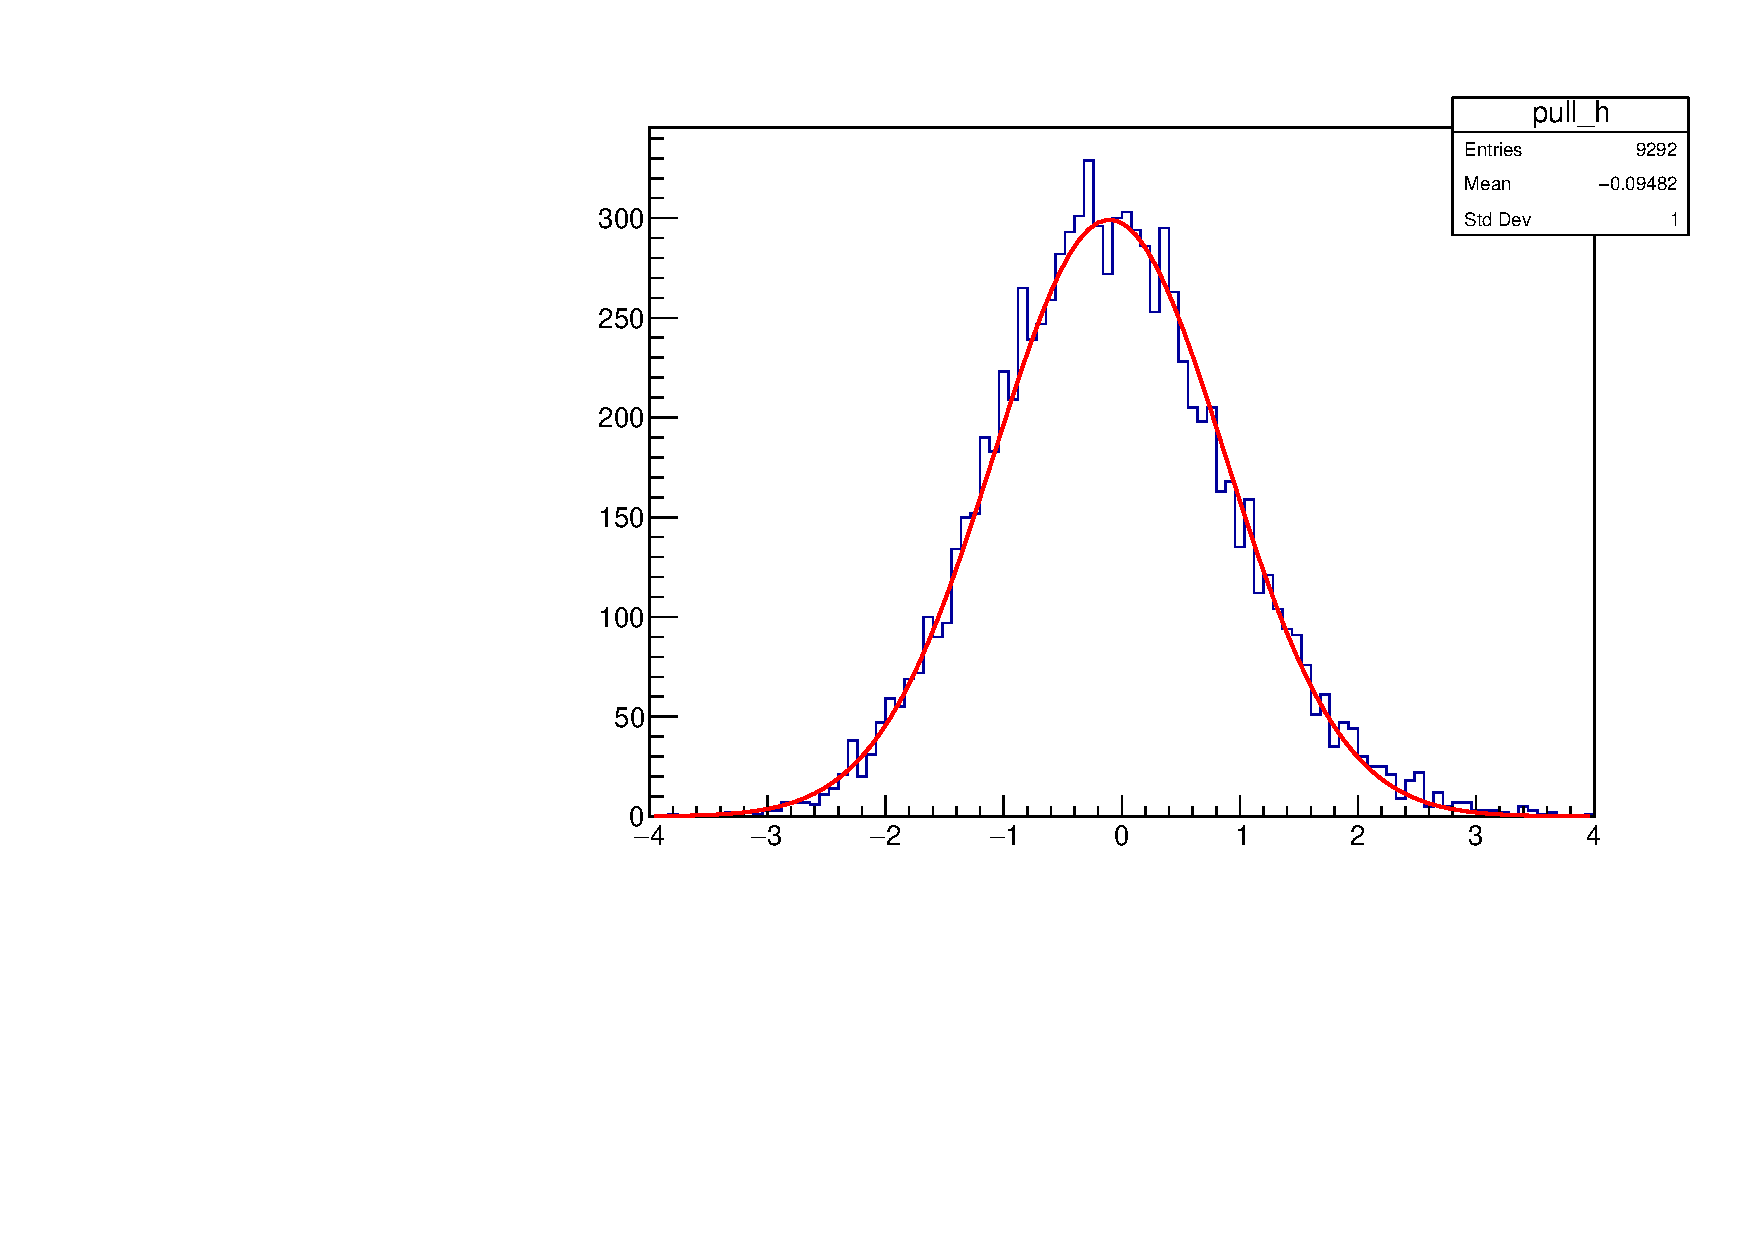
\includegraphics[width=1.0\textwidth]{Plots/signal_efficiency_pull_MuonUT_P3_ETA0.pdf}
      \caption*{$(p, \eta)$ bin $(3, 0)$}
    \end{subfigure}%
    \begin{subfigure}{0.45\textwidth}
      \centering
      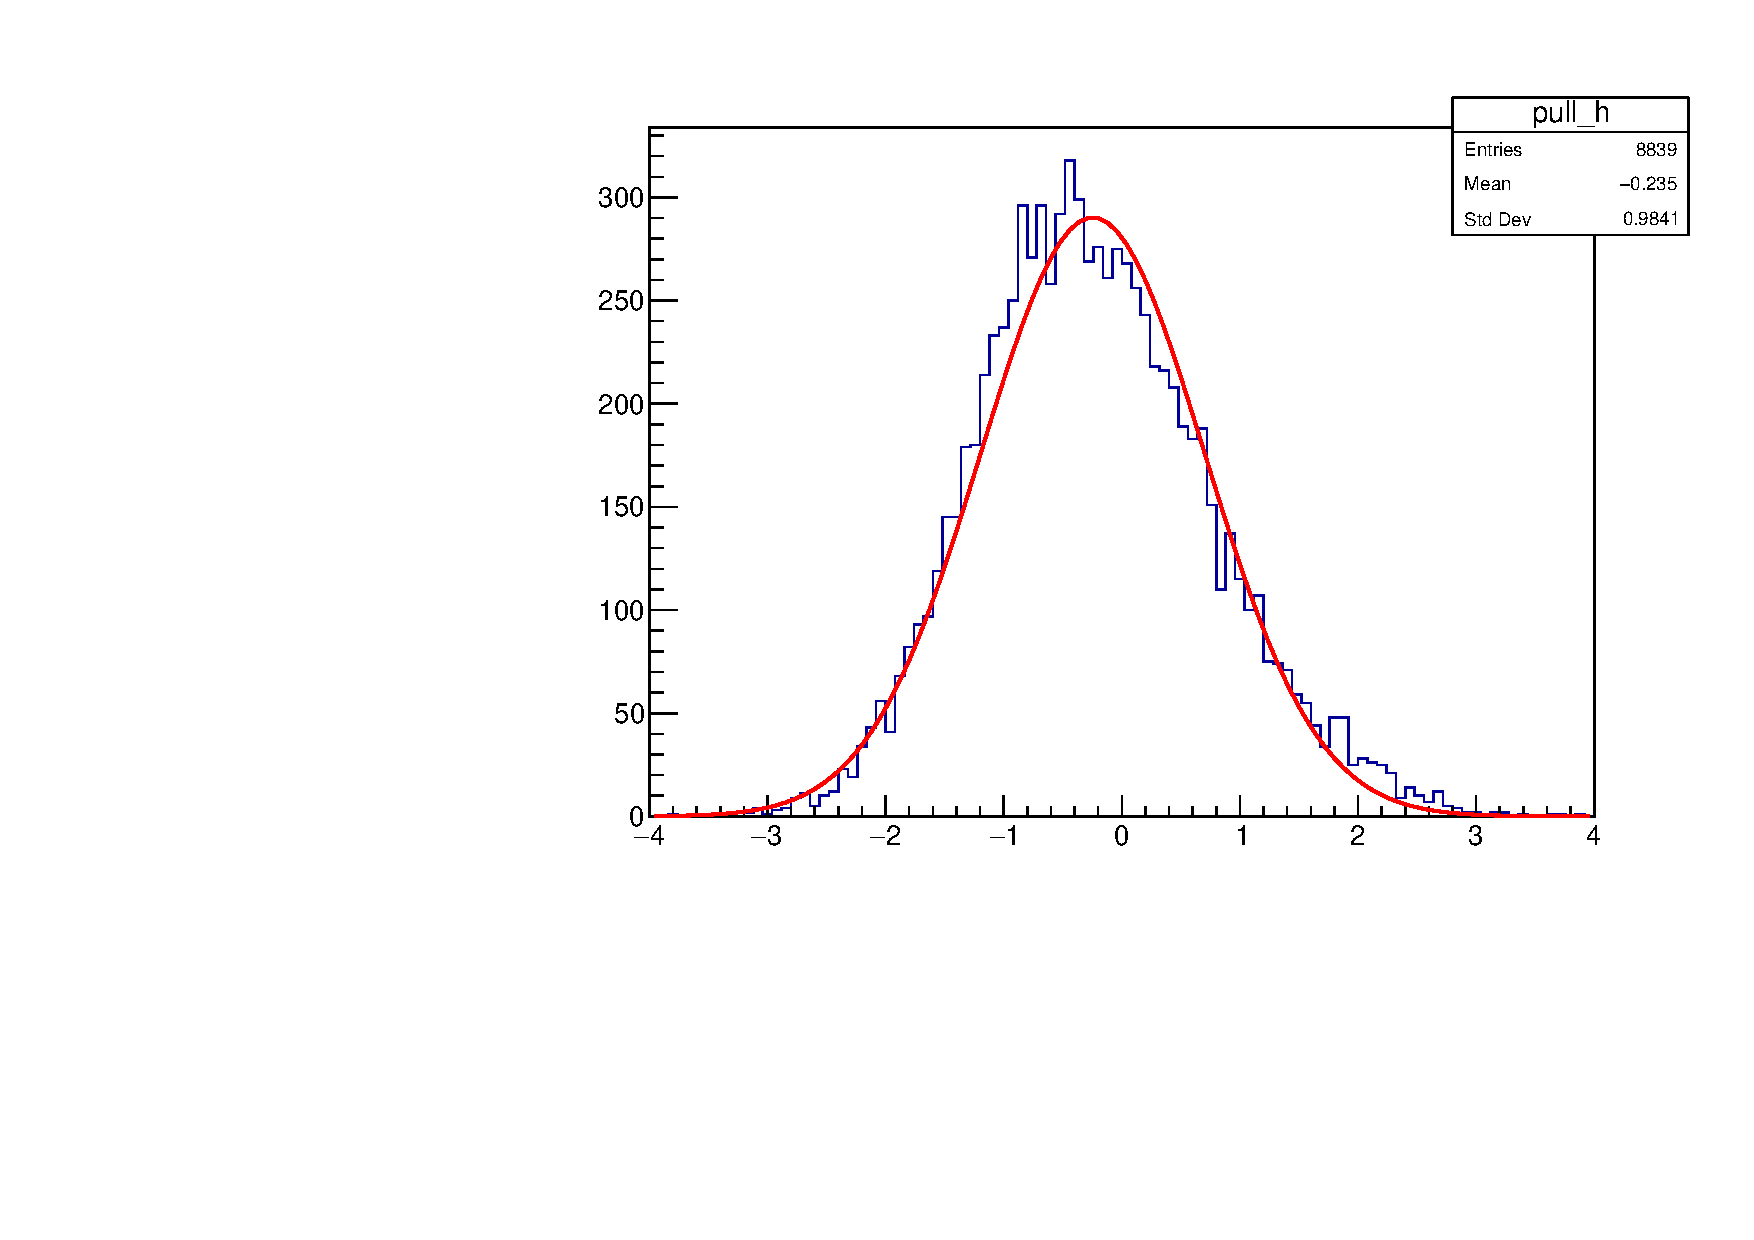
\includegraphics[width=1.0\textwidth]{Plots/signal_efficiency_pull_MuonUT_P2_ETA1.pdf}
      \caption*{$(p, \eta)$ bin $(2, 1)$}
    \end{subfigure}
    \vspace{-0.2cm}
  \end{figure}
  \begin{itemize}
    \item{In these bins we see reasonable behaviour (pulls are Gaussian shaped)}
    \item{Small negative bias, about $20$-$25\%$ of the statistical uncertainty}
  \end{itemize}
\end{frame}

\begin{frame}{Well-behaved fits}
  \vspace{0.0cm}
  \begin{figure}[htb]
    \centering
    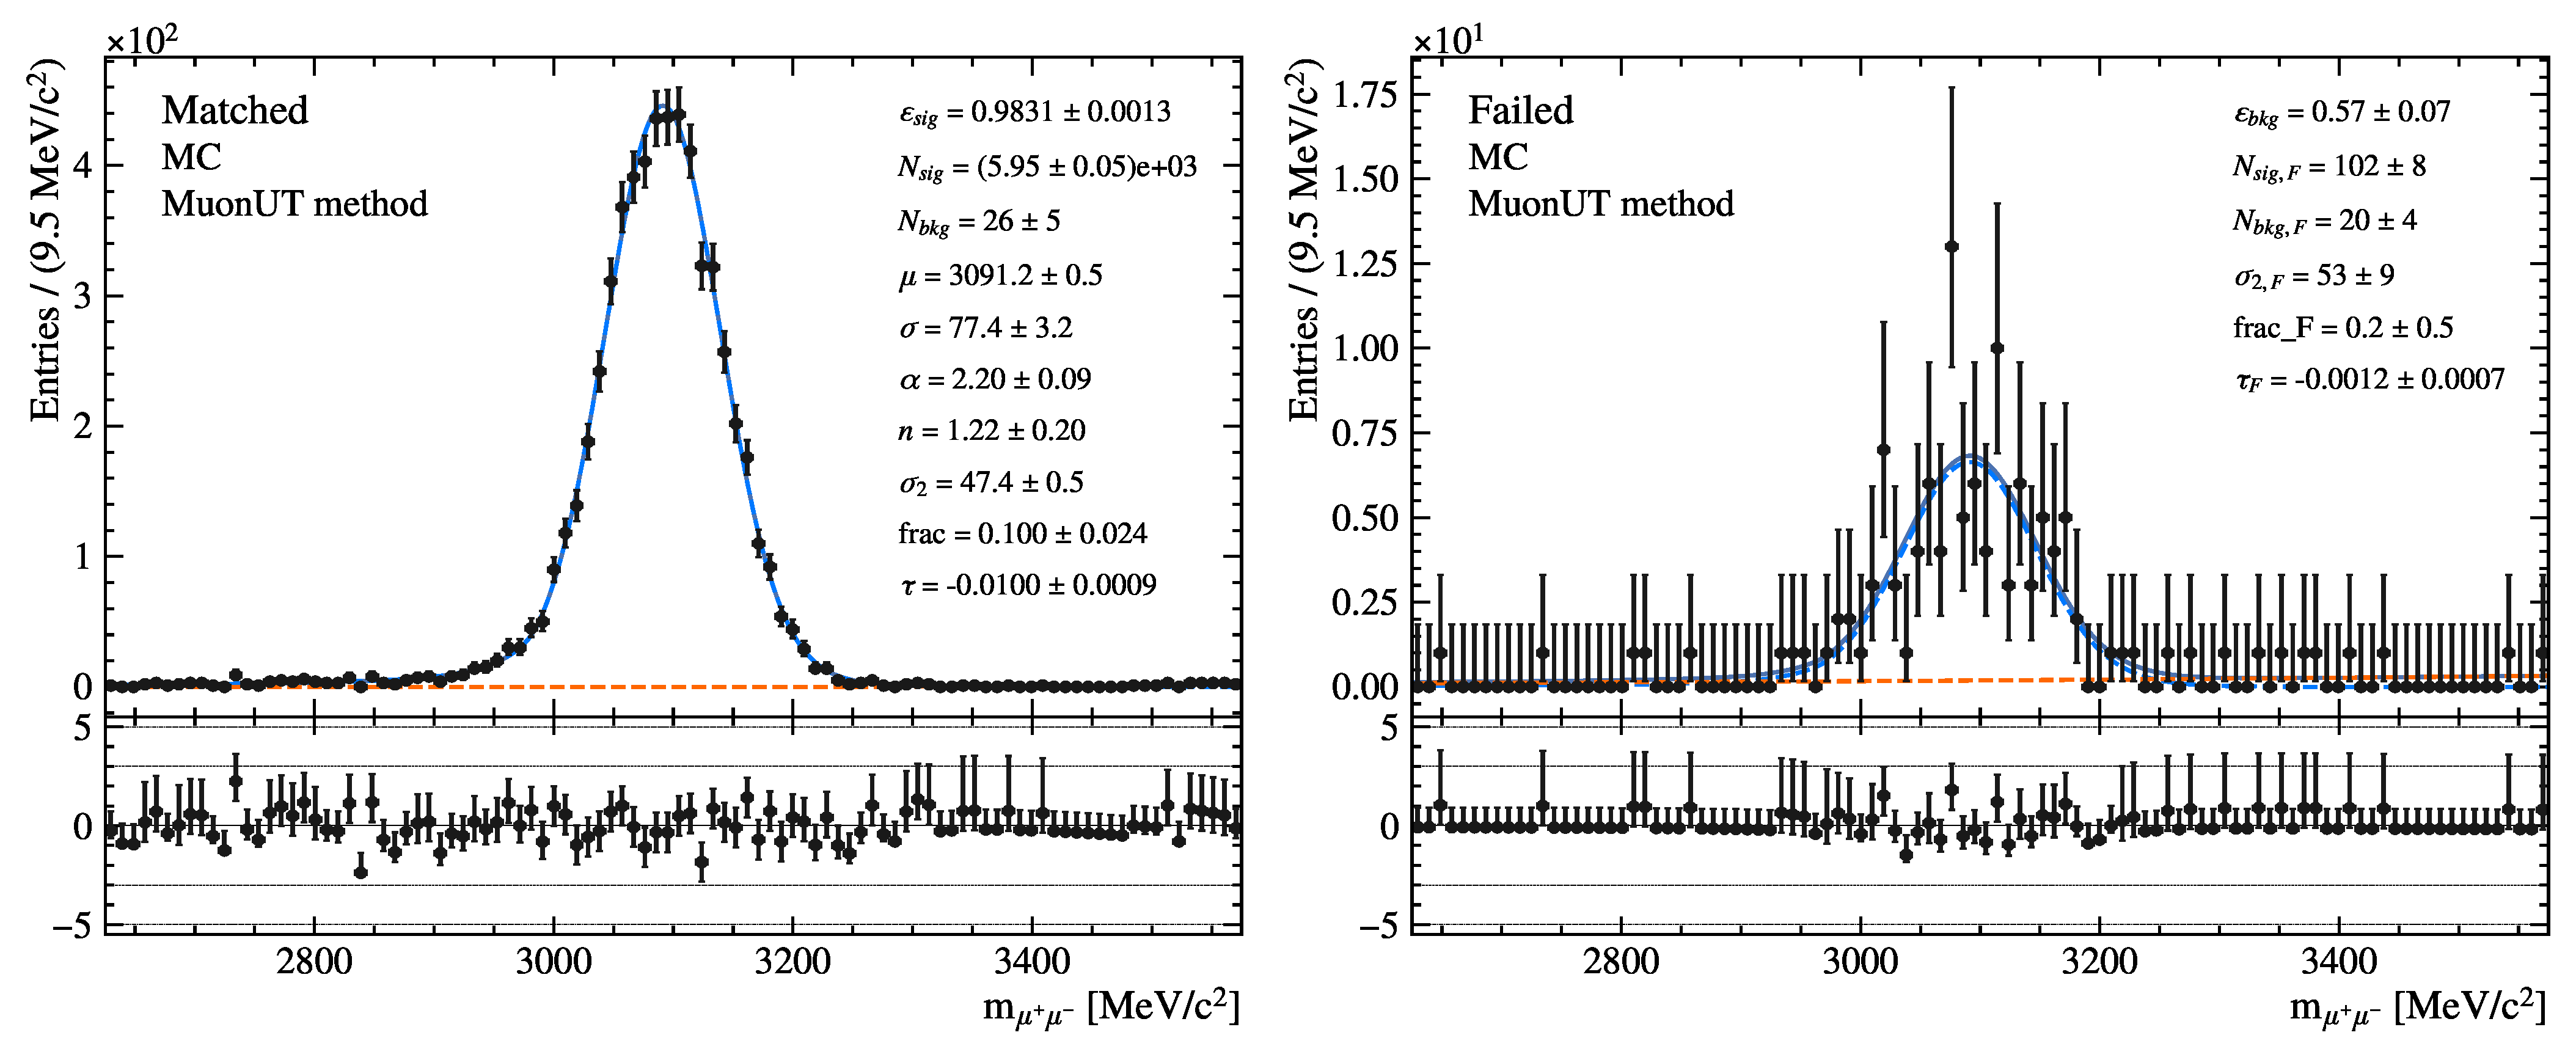
\includegraphics[width=0.65\textwidth]{Plots/MC_MuonUT_P_bin_3_ETA_bin_0_sim.pdf}
    \caption*{\small MuonUT $(p, \eta)$ bin $(3, 0)$}
  \end{figure}
  \vspace{-0.5cm}
  \begin{figure}[htb]
    \centering
    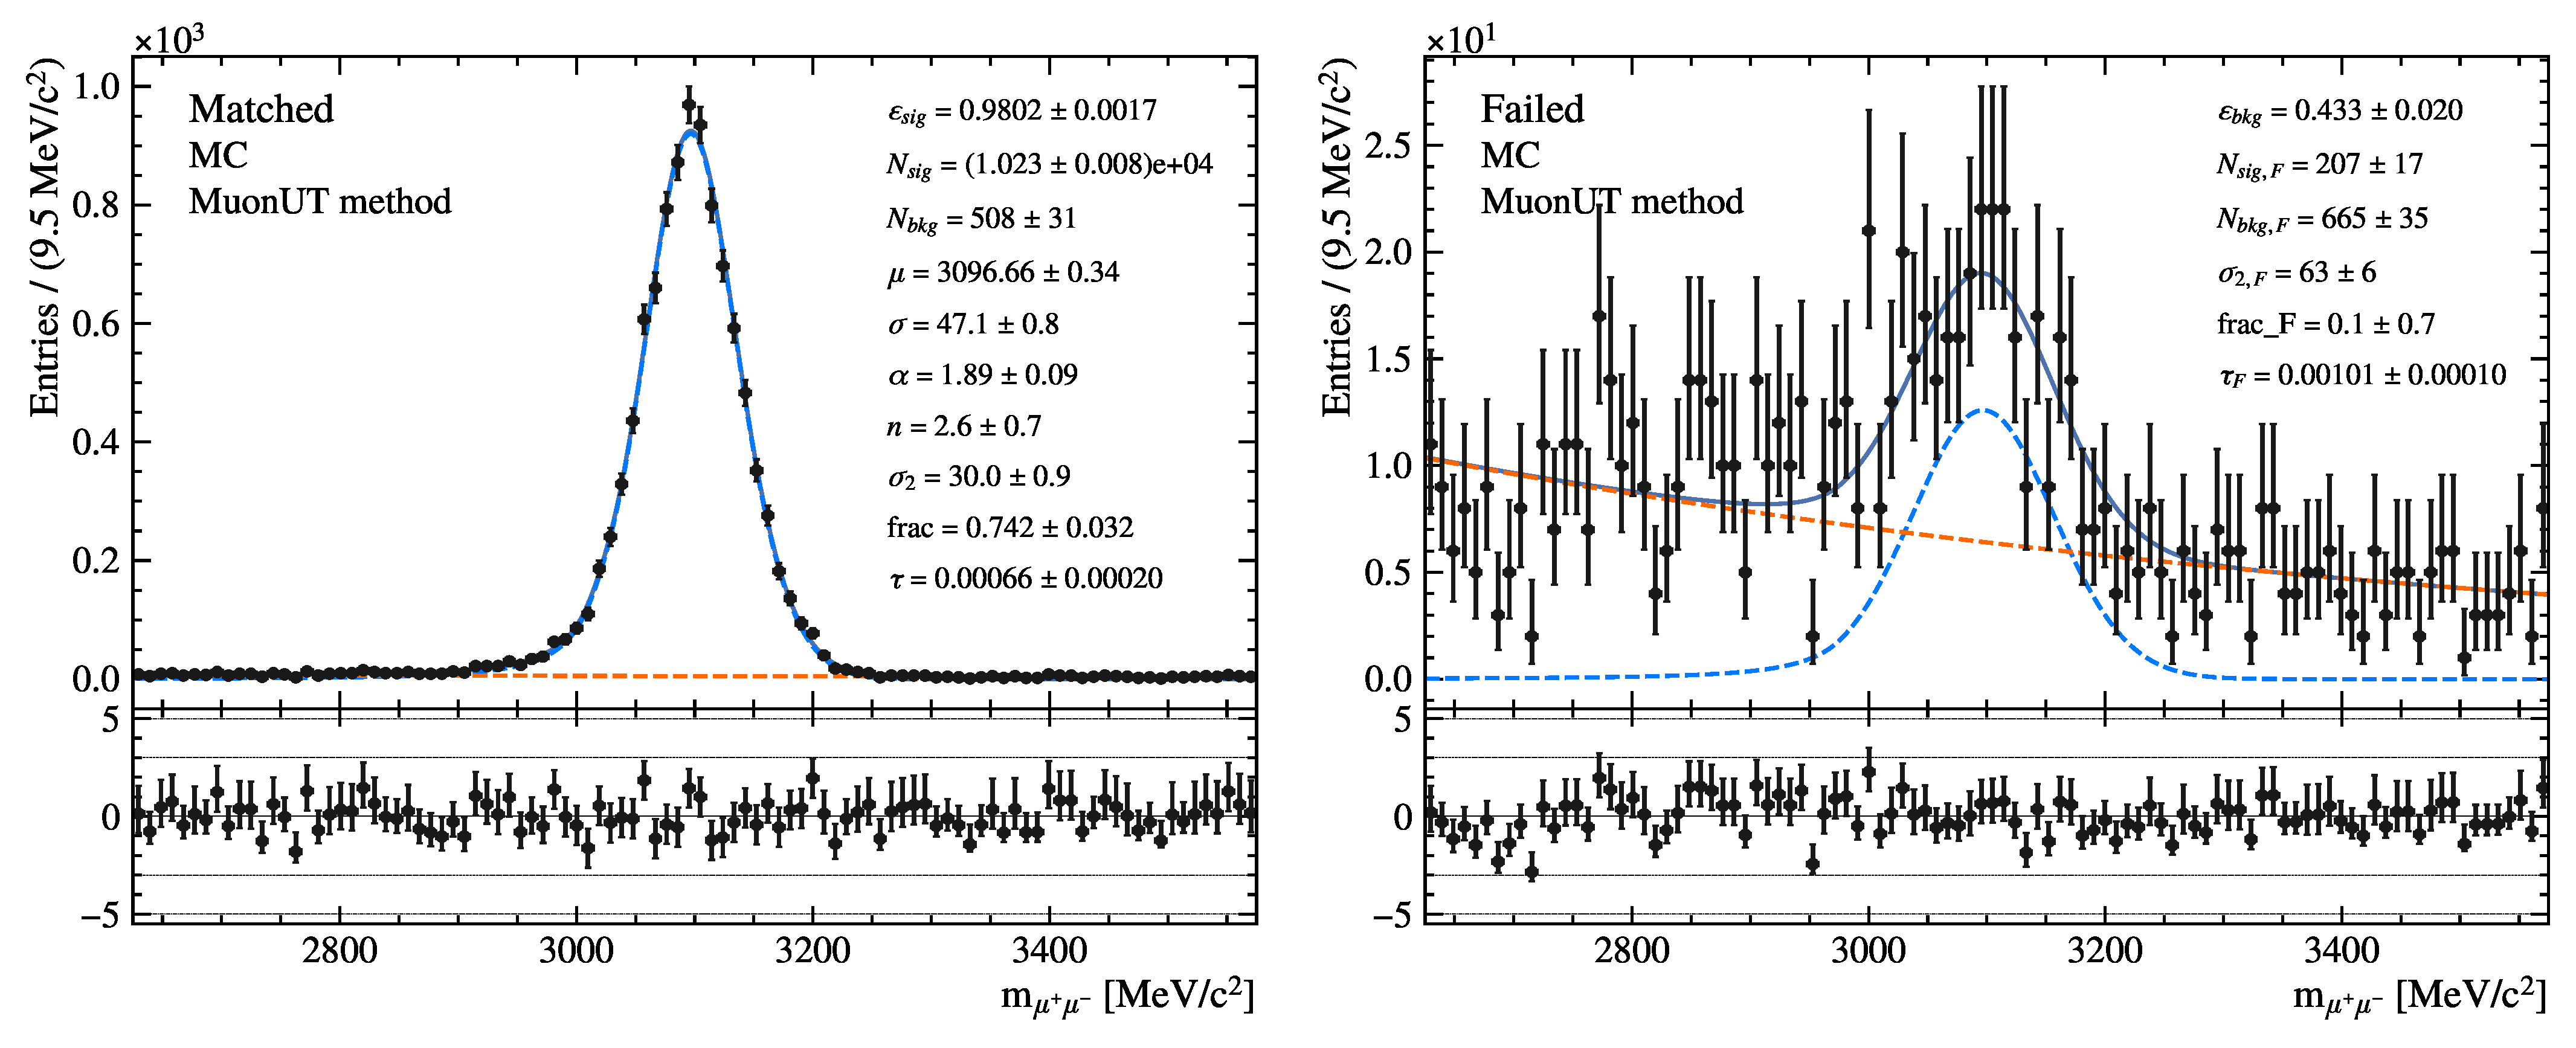
\includegraphics[width=0.65\textwidth]{Plots/MC_MuonUT_P_bin_2_ETA_bin_1_sim.pdf}
    \caption*{\small MuonUT $(p, \eta)$ bin $(2, 1)$}
  \end{figure}
\end{frame}

\begin{frame}{Biased fits}
  \vspace{0.0cm}
  \begin{figure}[htb]
    \centering
    \begin{subfigure}{0.45\textwidth}
      \centering
      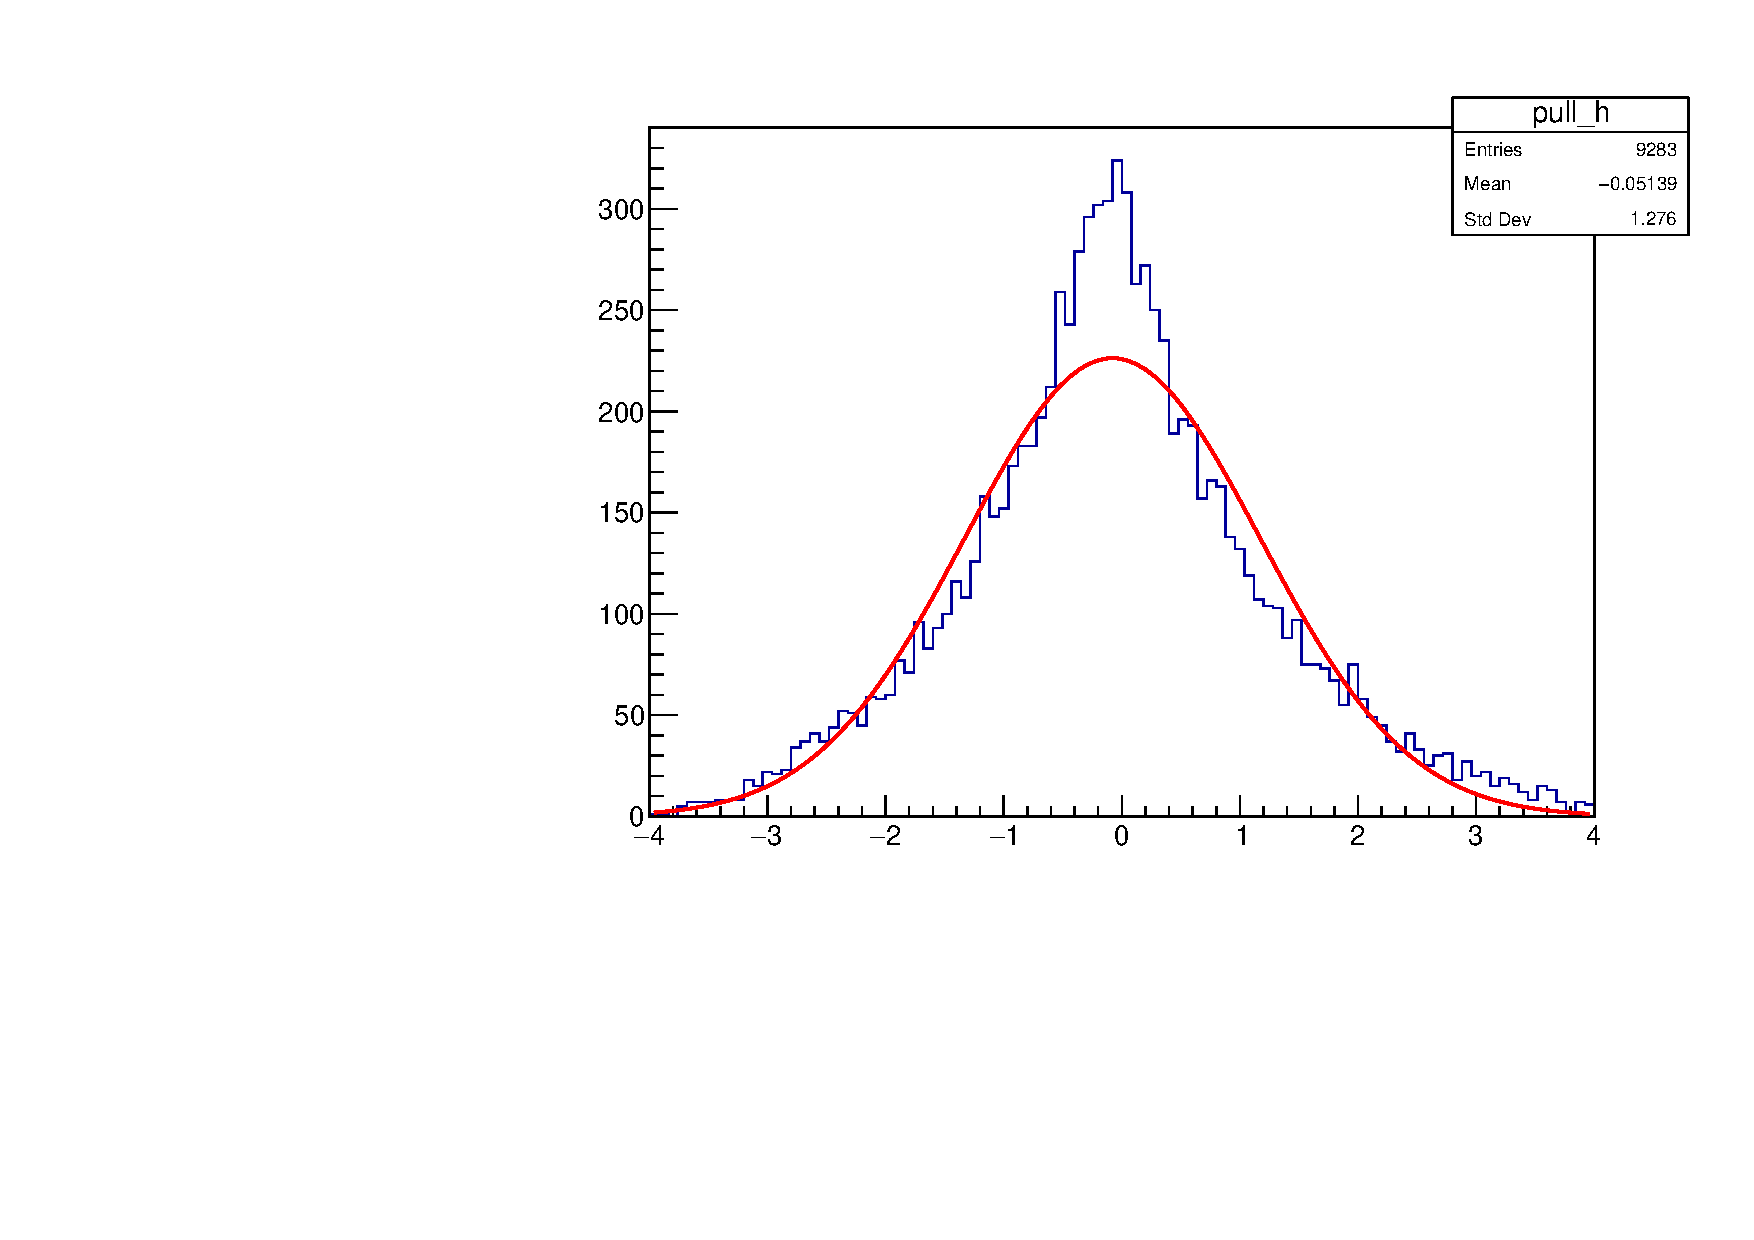
\includegraphics[width=1.0\textwidth]{Plots/signal_efficiency_pull_MuonUT_P2_ETA0.pdf}
      \caption*{$(p, \eta)$ bin $(2, 0)$}
    \end{subfigure}%
    \begin{subfigure}{0.45\textwidth}
      \centering
      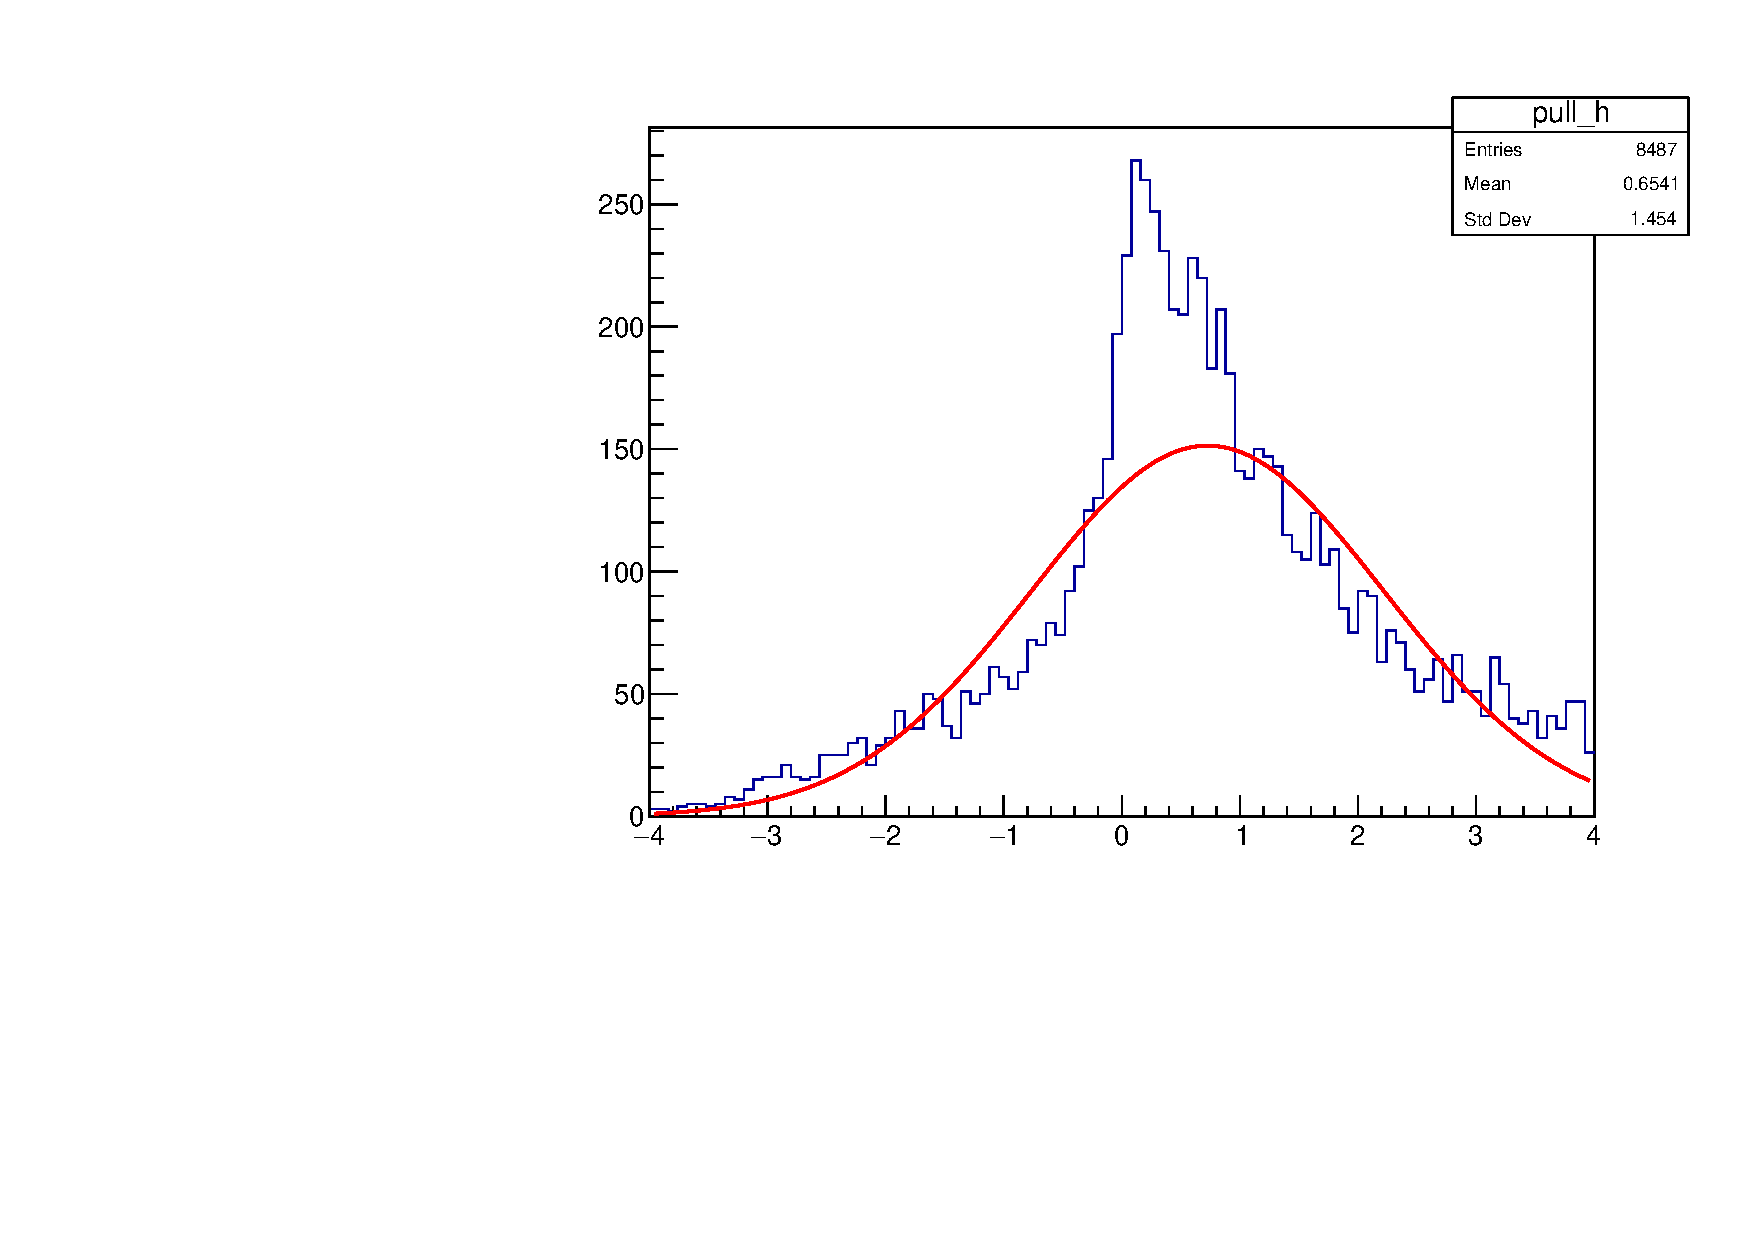
\includegraphics[width=1.0\textwidth]{Plots/signal_efficiency_pull_MuonUT_P4_ETA1.pdf}
      \caption*{$(p, \eta)$ bin $(4, 1)$}
    \end{subfigure}
    \vspace{-0.2cm}
  \end{figure}
  \begin{itemize}
    \item{Non-ideal statistical behaviour (pulls not Gaussian)}
    \item{Large tails and biases, actual uncertainties may be a lot larger}
  \end{itemize}
\end{frame}

\begin{frame}{Biased fits}
  \vspace{0.0cm}
  \begin{figure}[htb]
    \centering
    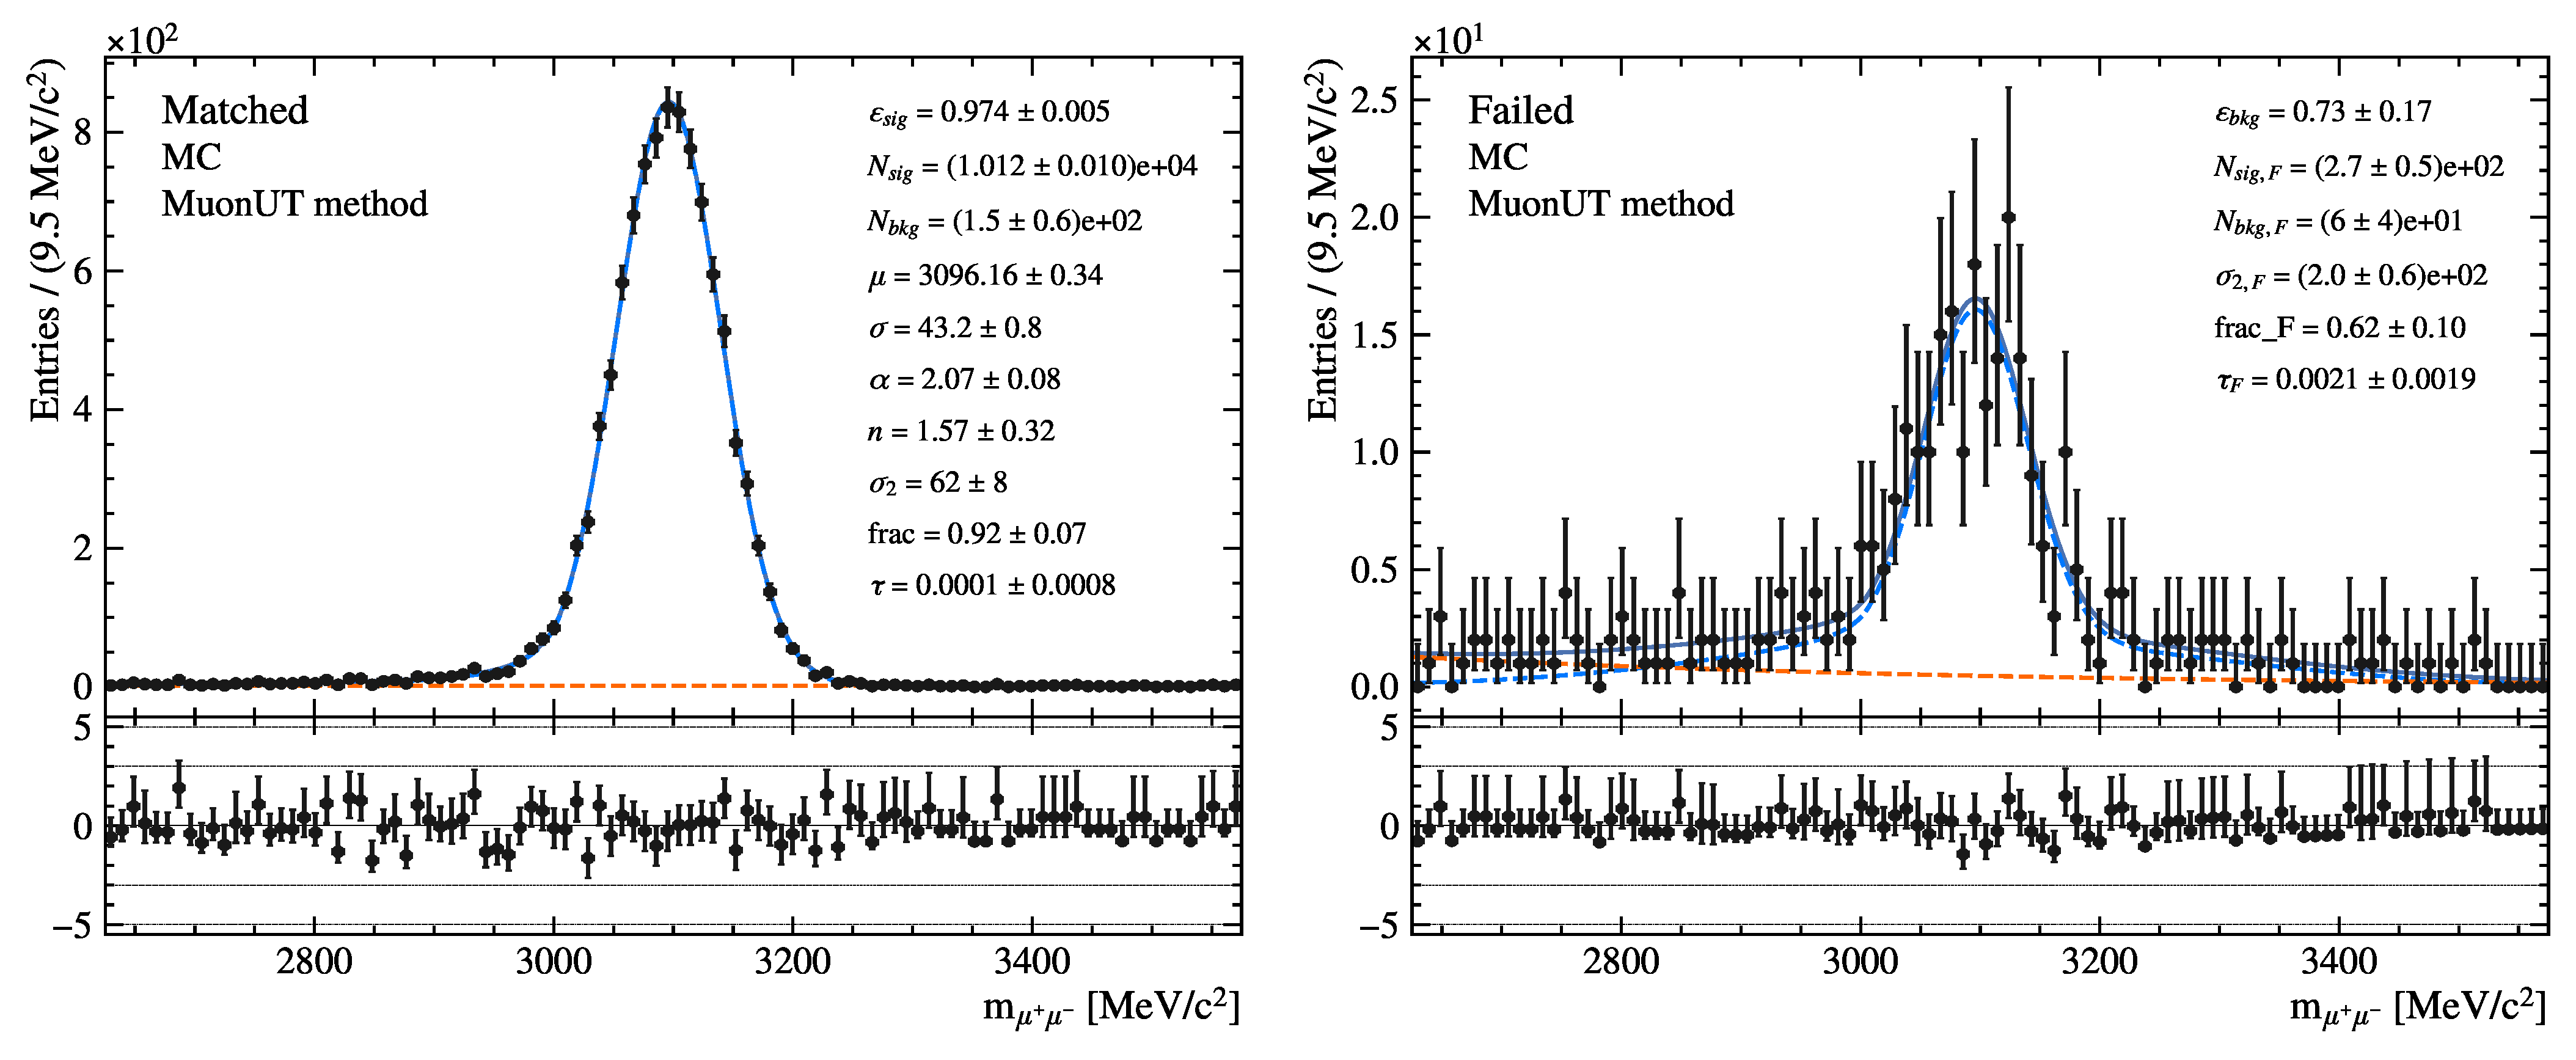
\includegraphics[width=0.65\textwidth]{Plots/MC_MuonUT_P_bin_2_ETA_bin_0_sim.pdf}
    \caption*{\small MuonUT $(p, \eta)$ bin $(2, 0)$}
  \end{figure}
  \vspace{-0.5cm}
  \begin{figure}[htb]
    \centering
    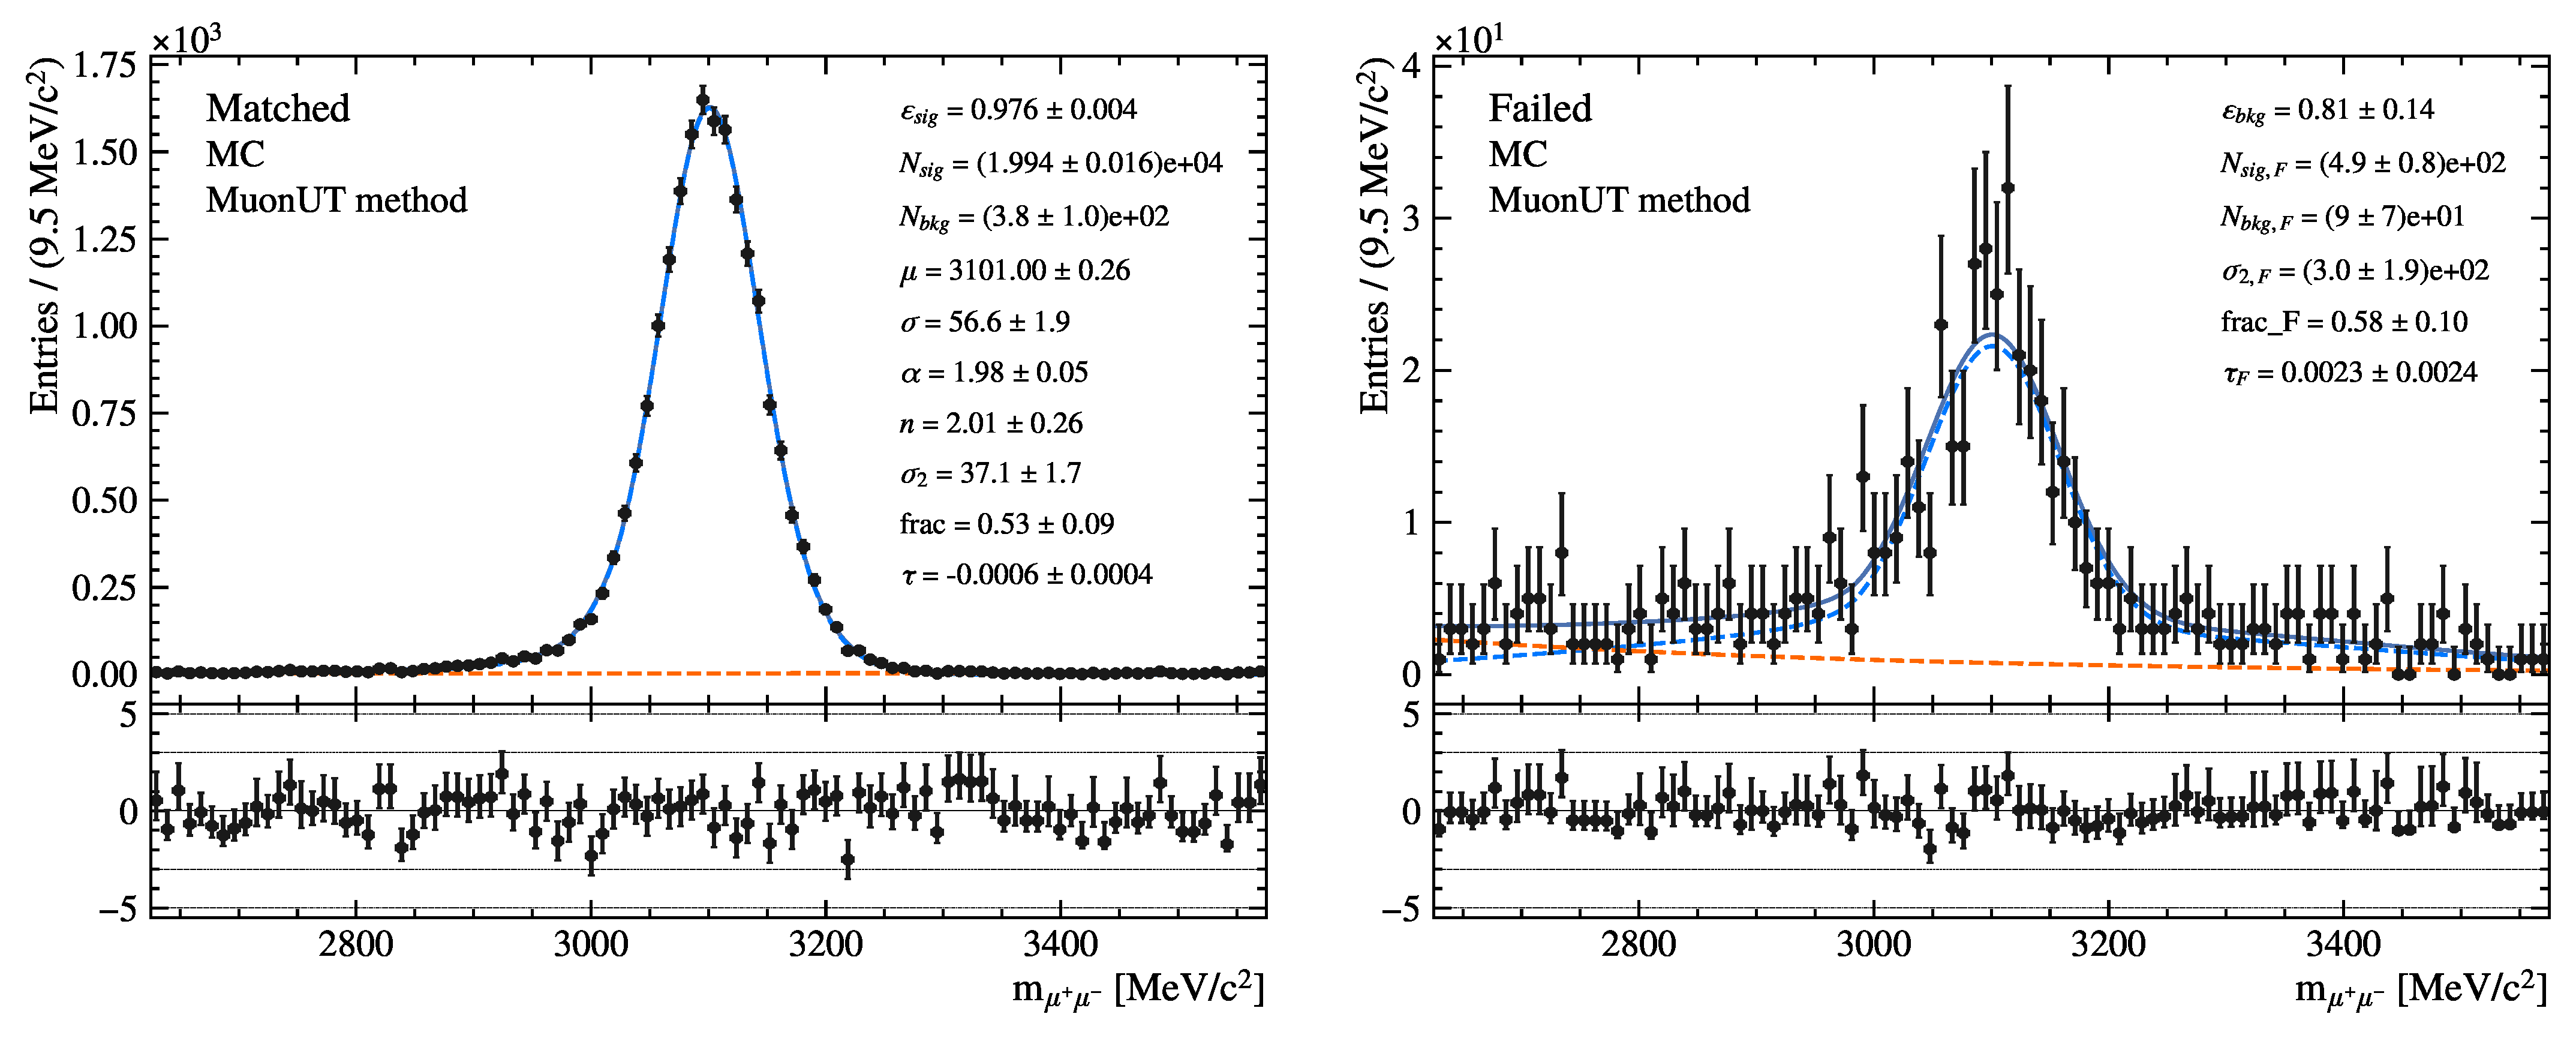
\includegraphics[width=0.65\textwidth]{Plots/MC_MuonUT_P_bin_4_ETA_bin_1_sim.pdf}
    \caption*{\small MuonUT $(p, \eta)$ bin $(4, 1)$}
  \end{figure}
\end{frame}

\begin{frame}{Fit biases}
  \vspace{0.0cm}
  \begin{itemize}
    \setlength\itemsep{0.0em}
    \item{My thoughts: Biases can occur when $\epsilon_{\rm track}$ is close to $1$...}
    \item{... but this can happen for both signal and background}
    \item{In fact I see a $90\%$ correlation between $\epsilon_{\rm track}$ in signal and background in some toys!}
  \end{itemize}
  \begin{center}
    \begin{tabular}{cccl}
      \hline
      $p$ bin & $\eta$ bin & Difference ($10^{-2}$)   & Gaussian? \\
      \hline
      $0$     & $0$        & $\phantom{-}0.4 \pm 1.1$ & Small tail \\
      $1$     & $0$        & $-0.5 \pm 0.2$           & Yes \\
      $2$     & $0$        & $-0.8 \pm 0.5$           & No, large tails \\
      $3$     & $0$        & $-1.5 \pm 0.1$           & Yes \\
      $4$     & $0$        & $-1.0 \pm 0.2$           & Yes \\
      $0$     & $1$        & $\phantom{-}3.2 \pm 1.9$ & No, small tail \\
      $1$     & $1$        & $\phantom{-}1.0 \pm 0.5$ & No, small tail \\
      $2$     & $1$        & $-0.9 \pm 0.2$           & Yes \\
      $3$     & $1$        & $\phantom{-}0.0 \pm 0.6$ & No, large tails \\
      $4$     & $1$        & $-0.7 \pm 0.4$           & No, large tails \\
      \hline
    \end{tabular}
  \end{center}
\end{frame}

\begin{frame}{Alternative background parameterisation}
  \vspace{0.0cm}
  \begin{itemize}
    \setlength\itemsep{1.0em}
    \item{In fits with highly correlated variables, alternative parameterisations usually help}
    \item{First attempt:}
    \begin{itemize}
      \item[-]{For signal, float $N_{\rm tot}$ and $\epsilon_{\rm track}$}
      \item[-]{For background, float $N_{\rm matched}$ and $N_{\rm failed}$ separately}
    \end{itemize}
    \item{Run same toy studies and check pull distributions}
  \end{itemize}
\end{frame}

\begin{frame}{Alternative background parameterisation}
  \vspace{0.0cm}
  \begin{figure}[htb]
    \centering
    \begin{subfigure}{0.45\textwidth}
      \centering
      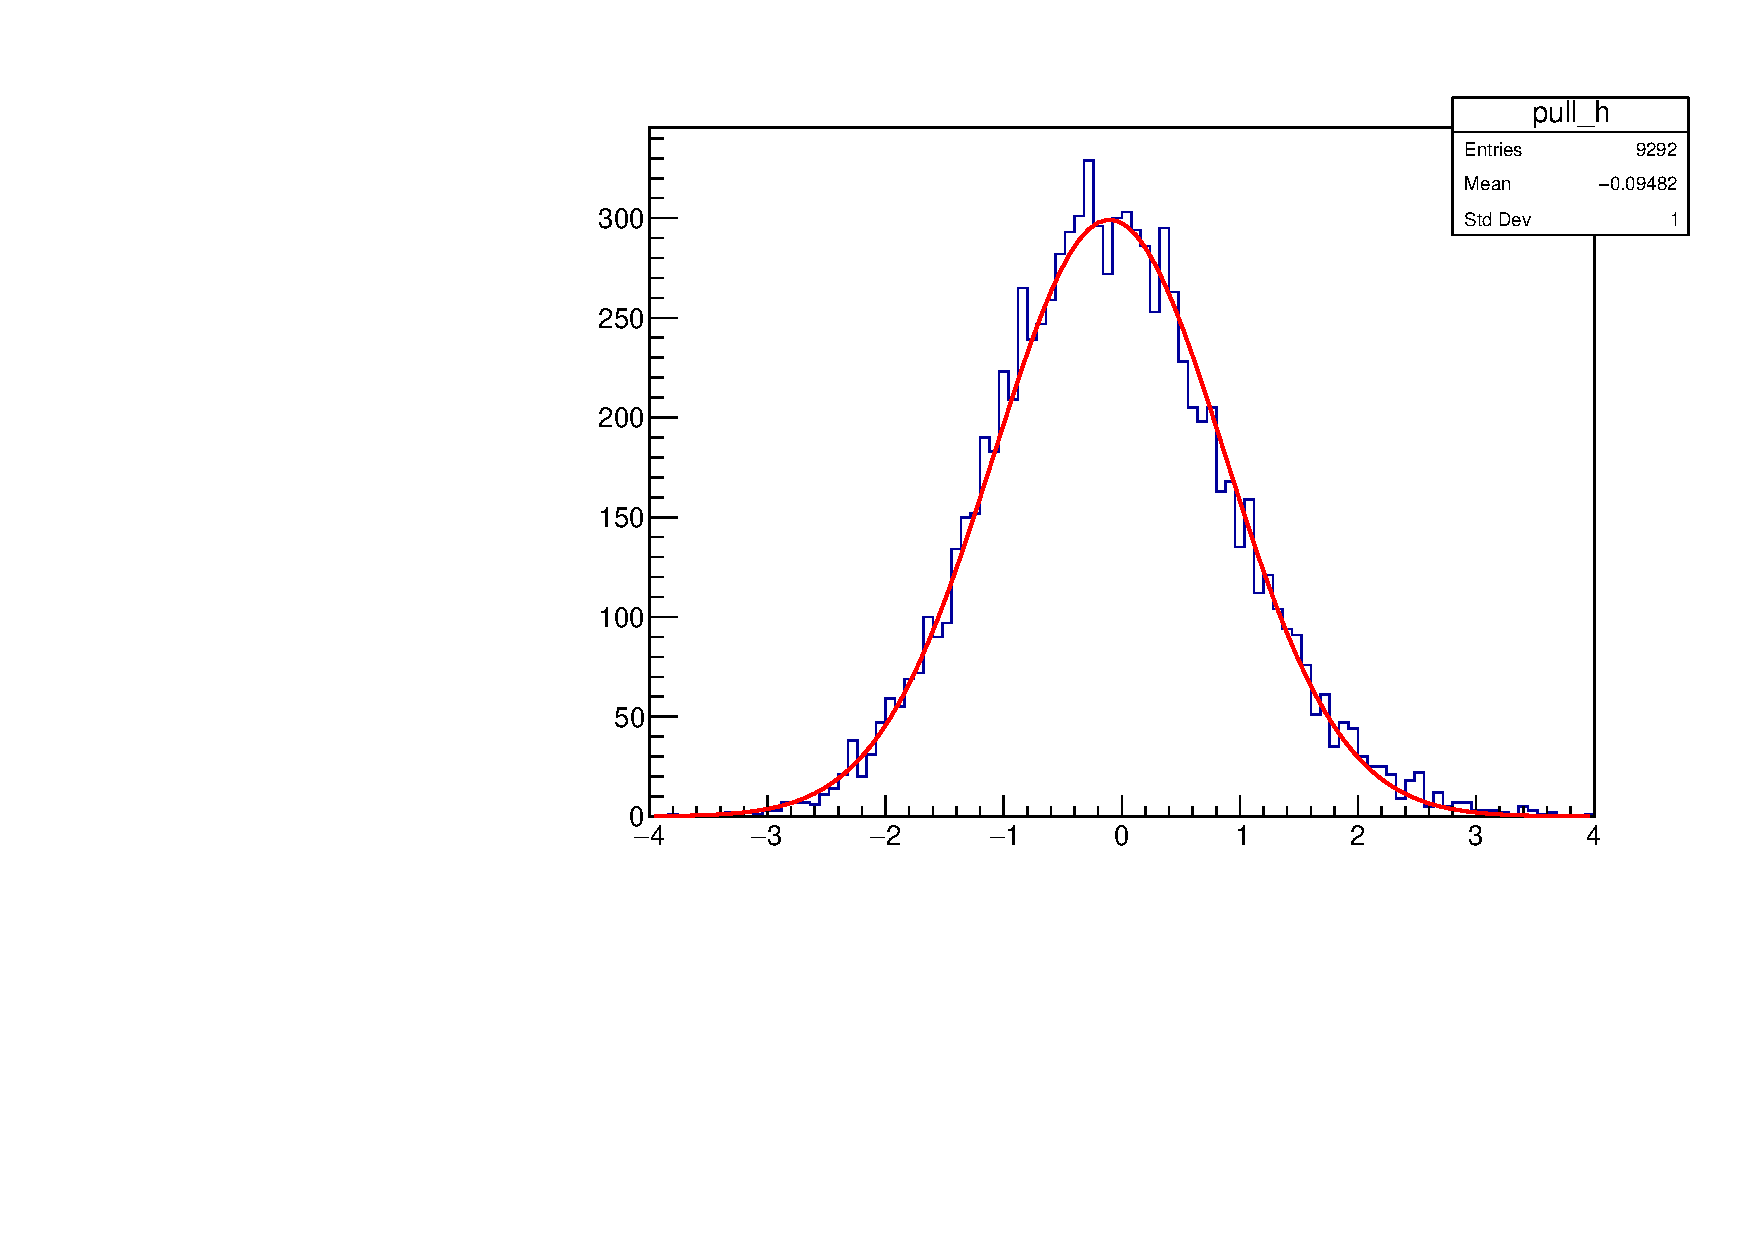
\includegraphics[width=1.0\textwidth]{Plots/signal_efficiency_pull_MuonUT_P3_ETA0.pdf}
      \caption*{Old parameterisation}
    \end{subfigure}%
    \begin{subfigure}{0.45\textwidth}
      \centering
      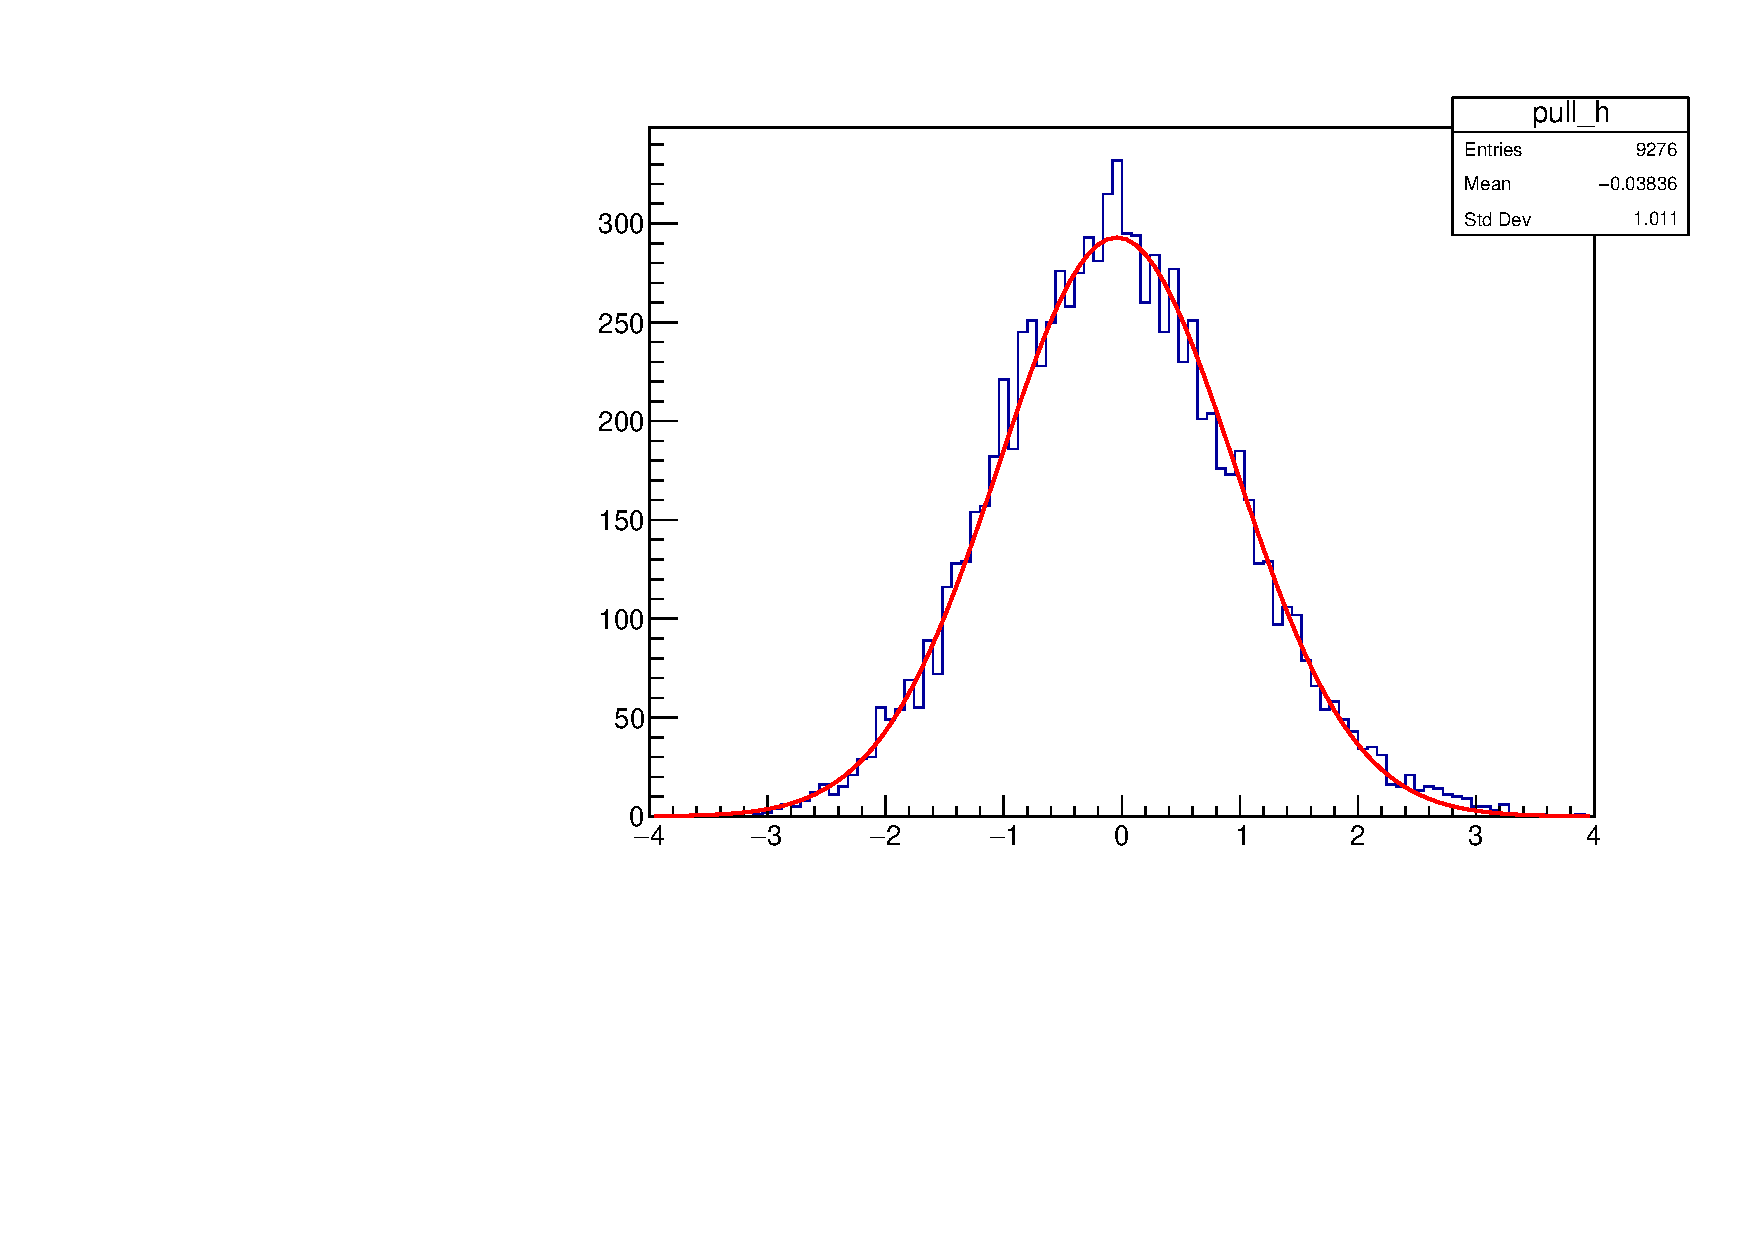
\includegraphics[width=1.0\textwidth]{Plots/signal_efficiency_pull_MuonUT_P3_ETA0_NoBkgEff.pdf}
      \caption*{New parameterisation}
    \end{subfigure}
    \vspace{-0.2cm}
    \caption*{$(p, \eta)$ bin $(3, 0)$}
  \end{figure}
  \begin{itemize}
    \item{Try floating the matched and failed yields directly}
    \item{Well behaved fits remain well behaved}
  \end{itemize}
\end{frame}

\begin{frame}{Alternative background parameterisation}
  \vspace{0.0cm}
  \begin{figure}[htb]
    \centering
    \begin{subfigure}{0.45\textwidth}
      \centering
      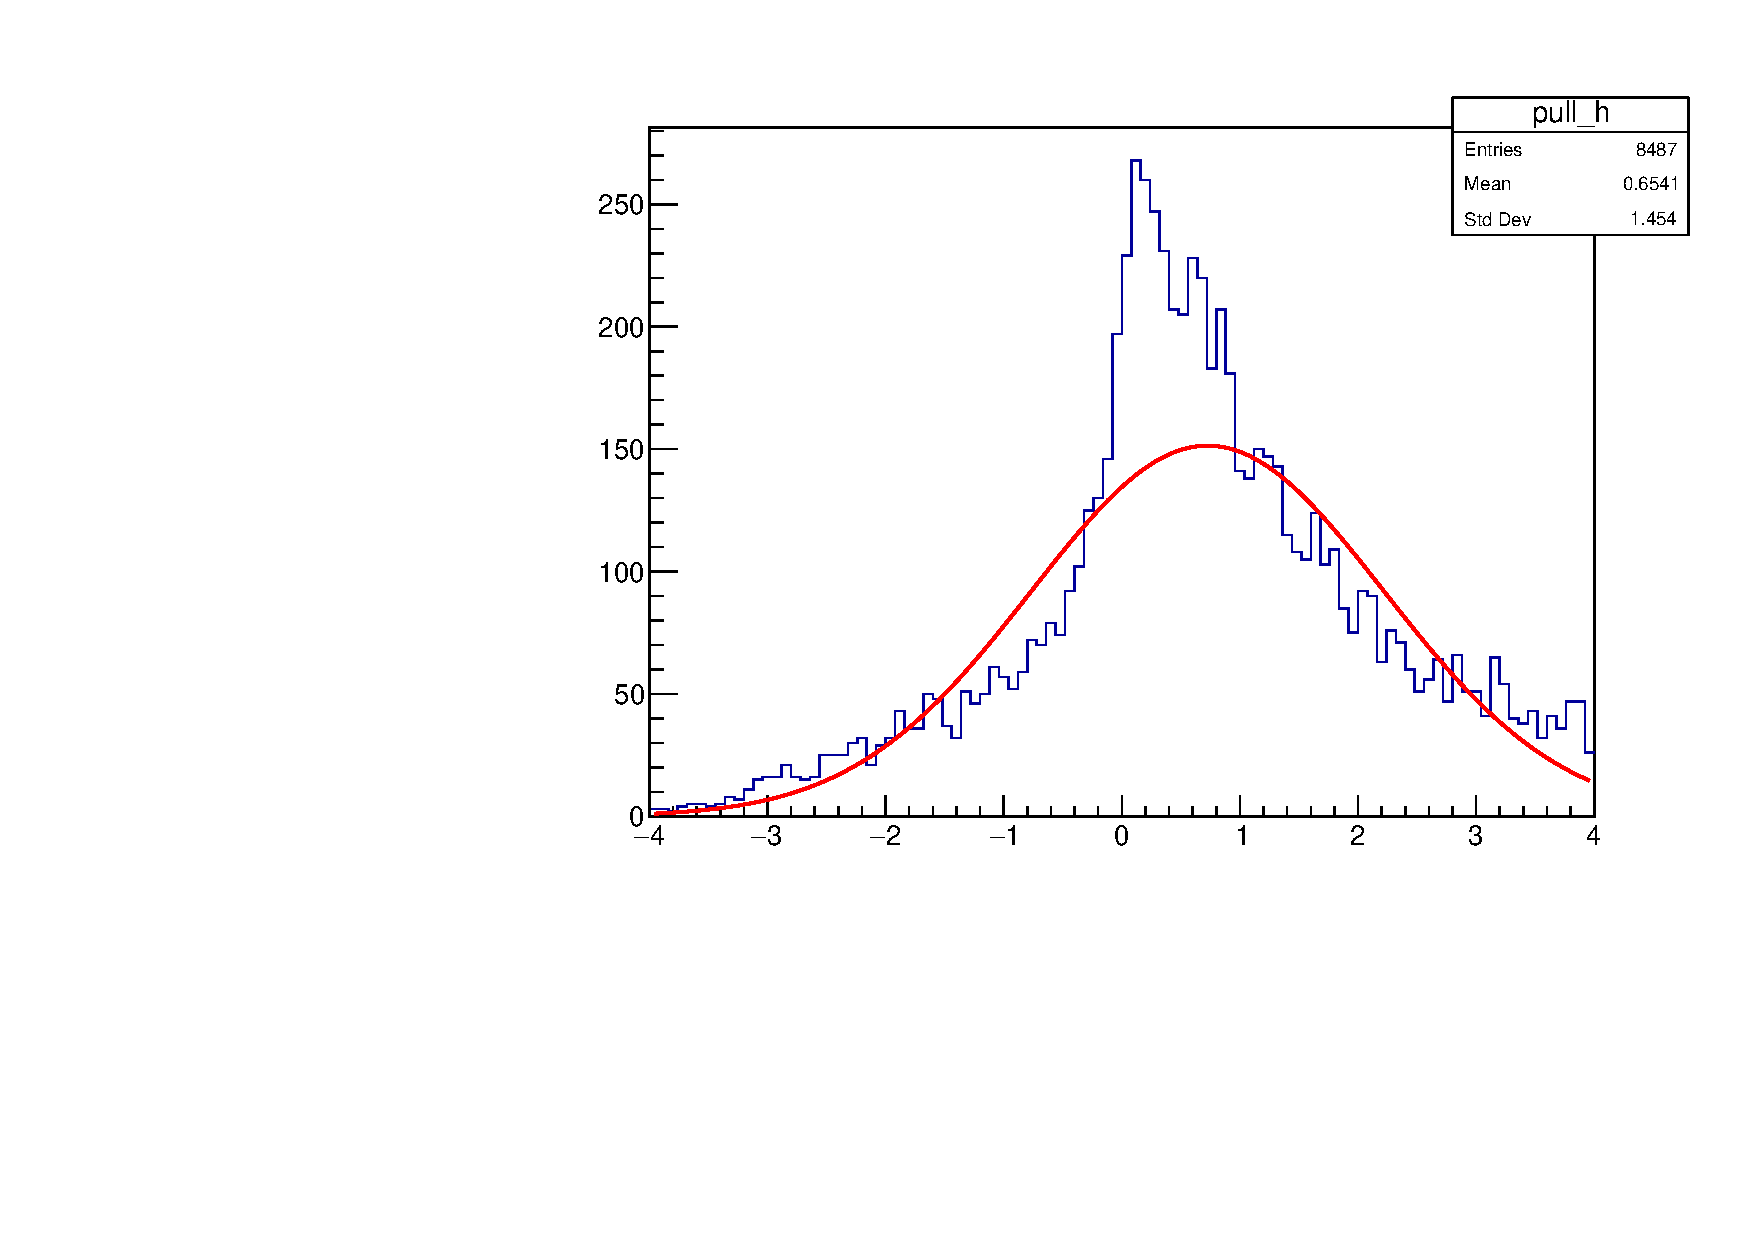
\includegraphics[width=1.0\textwidth]{Plots/signal_efficiency_pull_MuonUT_P4_ETA1.pdf}
      \caption*{Old parameterisation}
    \end{subfigure}%
    \begin{subfigure}{0.45\textwidth}
      \centering
      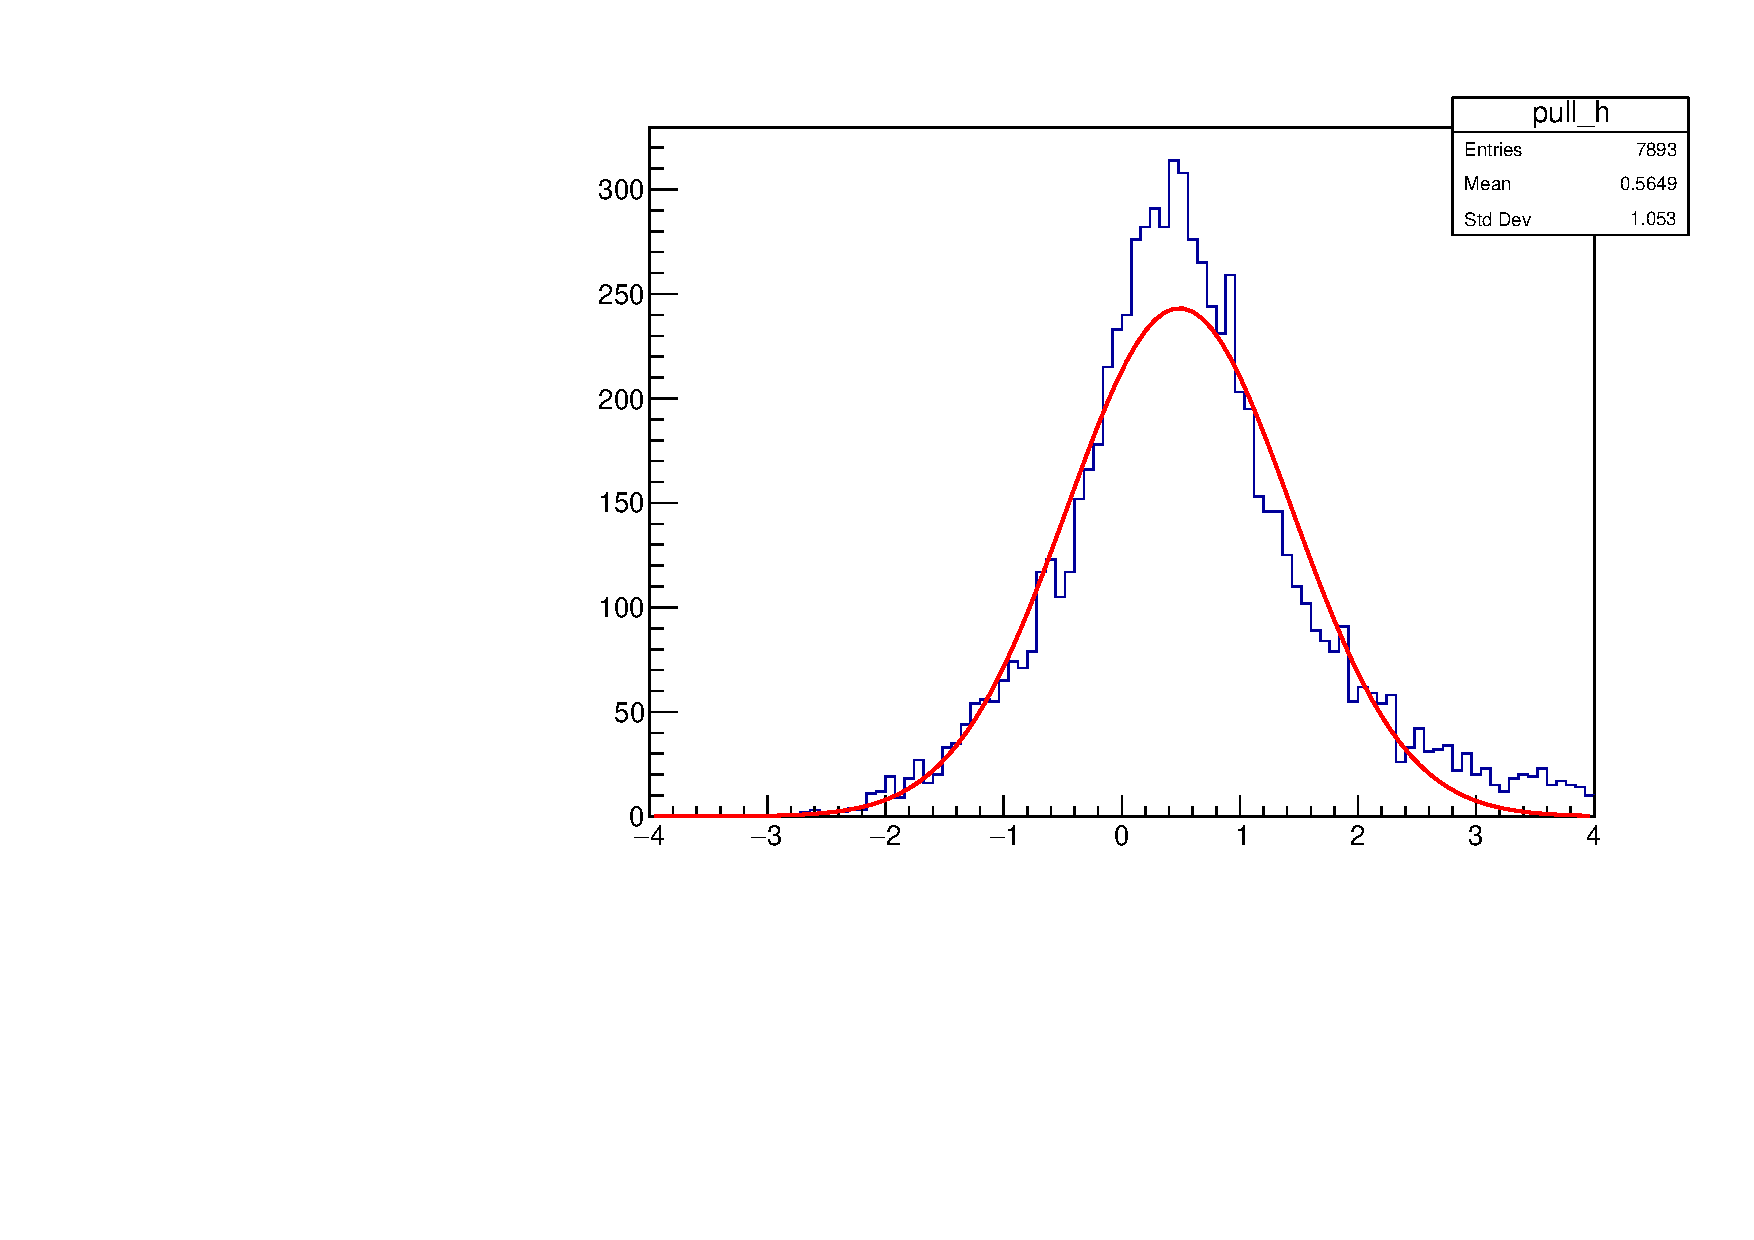
\includegraphics[width=1.0\textwidth]{Plots/signal_efficiency_pull_MuonUT_P4_ETA1_NoBkgEff.pdf}
      \caption*{New parameterisation}
    \end{subfigure}
    \vspace{-0.2cm}
    \caption*{$(p, \eta)$ bin $(4, 1)$}
  \end{figure}
  \begin{itemize}
    \item{Try floating the matched and failed yields directly}
    \item{Statistical behaviour seems to improve in some fits!}
  \end{itemize}
\end{frame}

\begin{frame}{Summary and next steps}
  \vspace{0.0cm}
  \begin{itemize}
    \setlength\itemsep{1.0em}
    \item{I checked the impact of fit biases in the MuonUT method}
    \begin{enumerate}
      \setlength\itemsep{0.3em}
      \item{In some bins, fit biases could be significant}
      \item{For a meaningful comparison, the MuonUT methods needs to:}
      \begin{itemize}
        \item[-]{Have small fit biases}
        \item[-]{Converge with correct uncertainties without need to rerun fit}
      \end{itemize}
      \item{Only MC studied so far, but I suspect similar effects are present in data}
    \end{enumerate}
    \item{Next steps: Do the same checks in data}
  \end{itemize}
  \vspace{0.3cm}
  \begin{center}
    \Huge Thanks for listening!
  \end{center}
\end{frame}

\end{document}
